\newpage
\appendix
\section{Graphical Comparison of the Background Estimations}
\label{app:graphical}
The efforts described in works~\cite{AN2012:248,AN2012:255,AN2012:256} are summarised for 
a review in the plots presented in this section. If not stated explicitly, the black color in the plots corresponds to 
a Ref.~\cite{AN2012:248}, the red color to a Ref.~\cite{AN2012:255}, and the blue color to a Ref.~\cite{AN2012:256}.
While for the tri-lepton processes without a tau three results are compared, for channels with a tau present
contribution were made by two out of three works which are presented in the plots.
%==========================================================================================
\begin{figure}[htp]
\begin{center}
\subfigure[]
{\label{fig:rare_3l}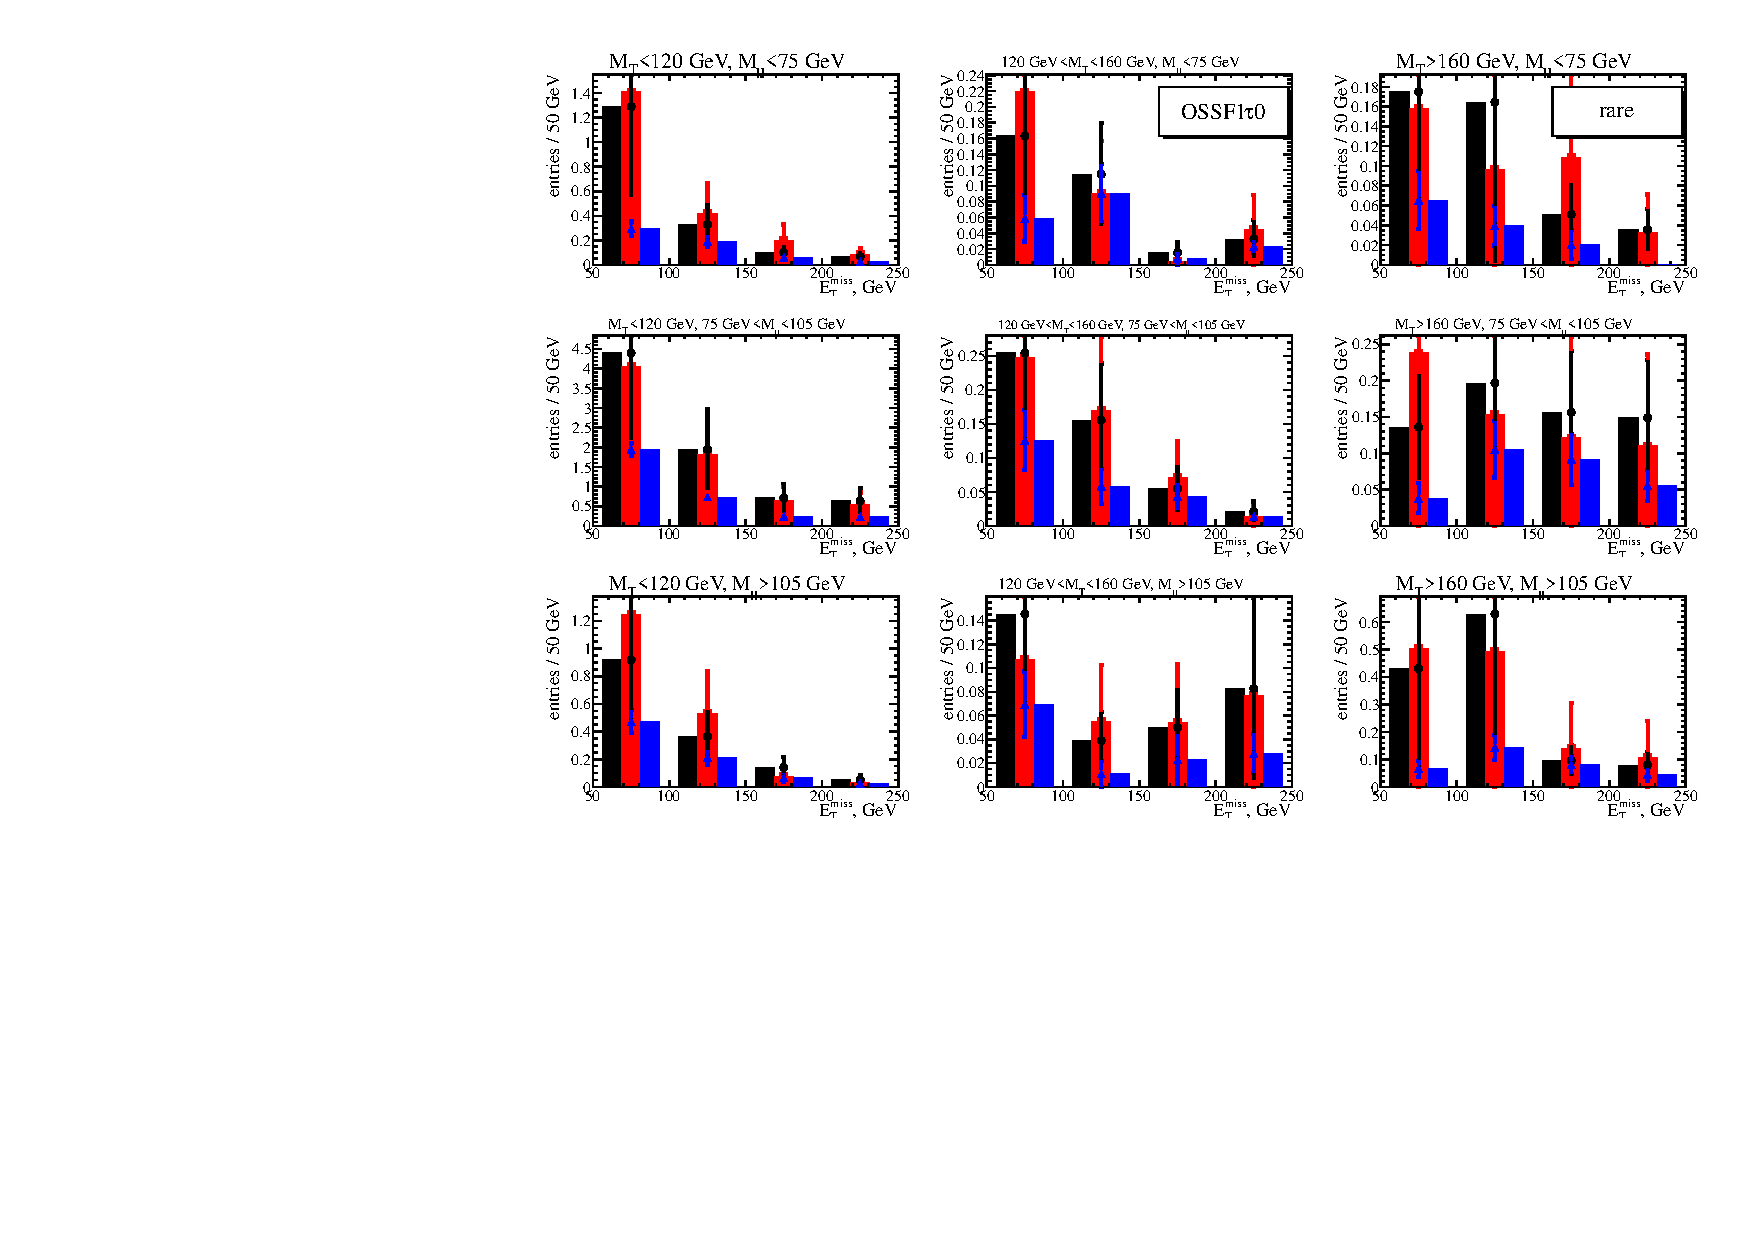
\includegraphics[width=1.0\textwidth]{plots/3lbkg/rare_ossf1tau0A.pdf}} \\
\subfigure[]
{\label{fig:rare_noOSSF}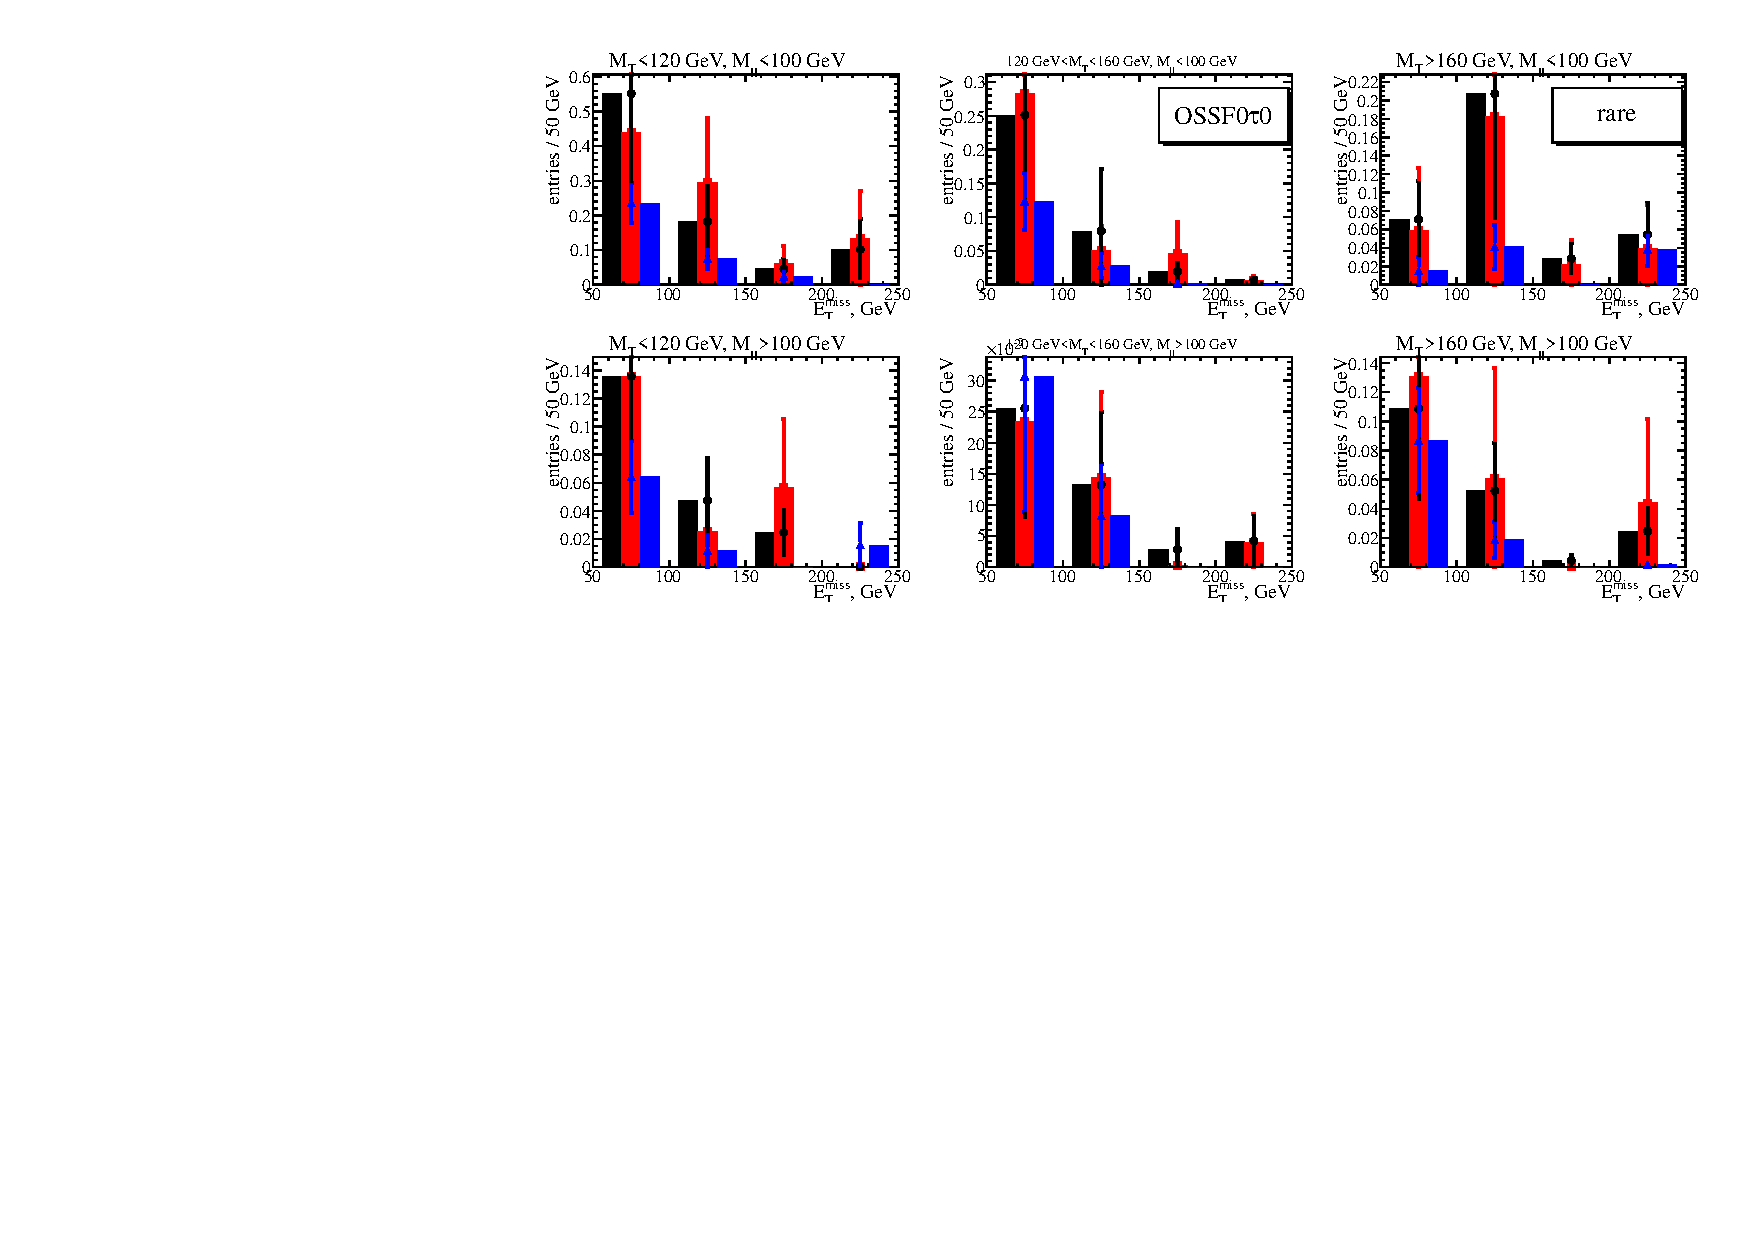
\includegraphics[width=1.0\textwidth]{plots/3lbkg/rare_ossf0tau0A.pdf}} \\
\caption{Comparison of the Rare SM contribution.  Blue histograms from Ref.~\cite{AN2012:256} do not fully take into account 
all the processes therefore their contribution is excluded from the final combination.}
\label{fig:rare1}
\end{center}
\end{figure}
%==========================================================================================
%==========================================================================================
\begin{figure}[htp]
\begin{center}
\subfigure[]
{\label{fig:rare_SStau}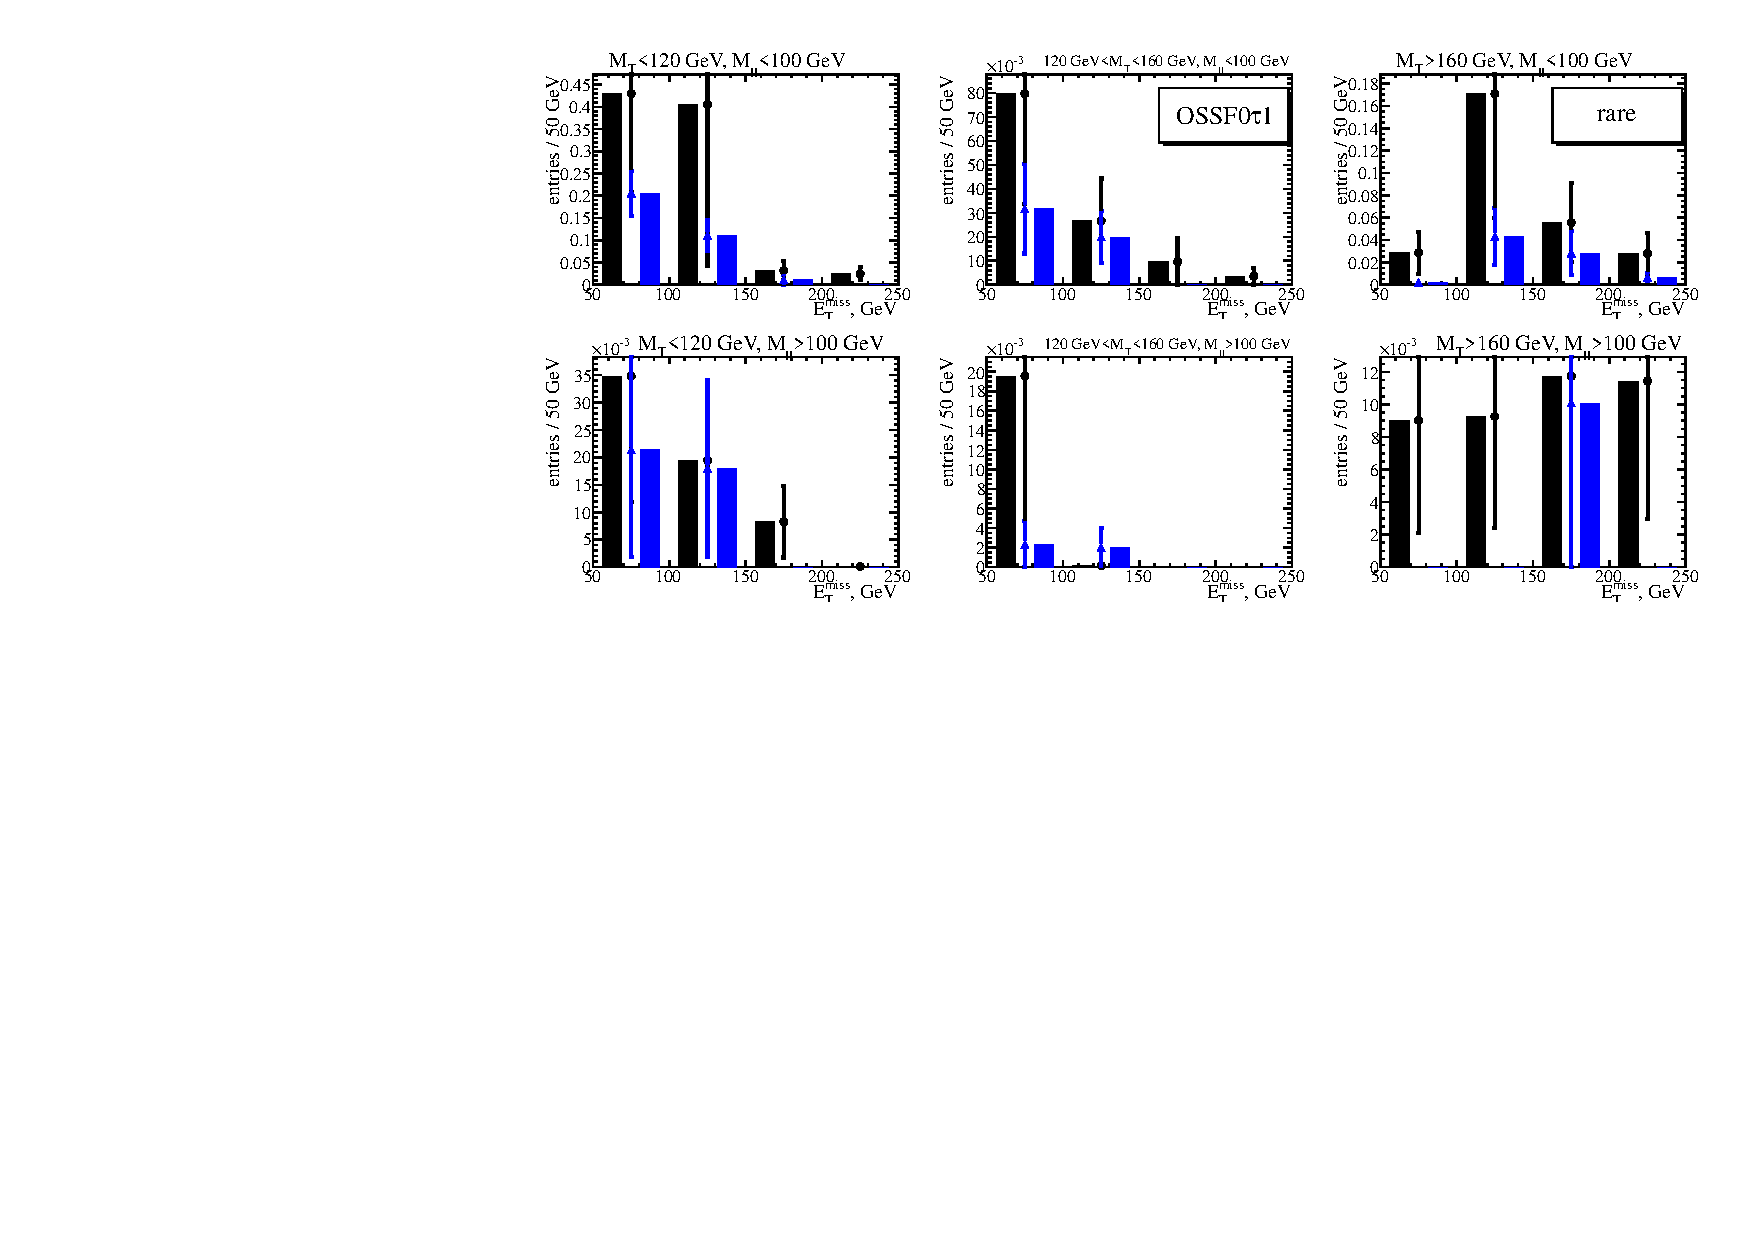
\includegraphics[width=1.0\textwidth]{plots/3lbkg/rare_ossf0tau1A.pdf}} \\
\subfigure[]
{\label{fig:rare_OStau}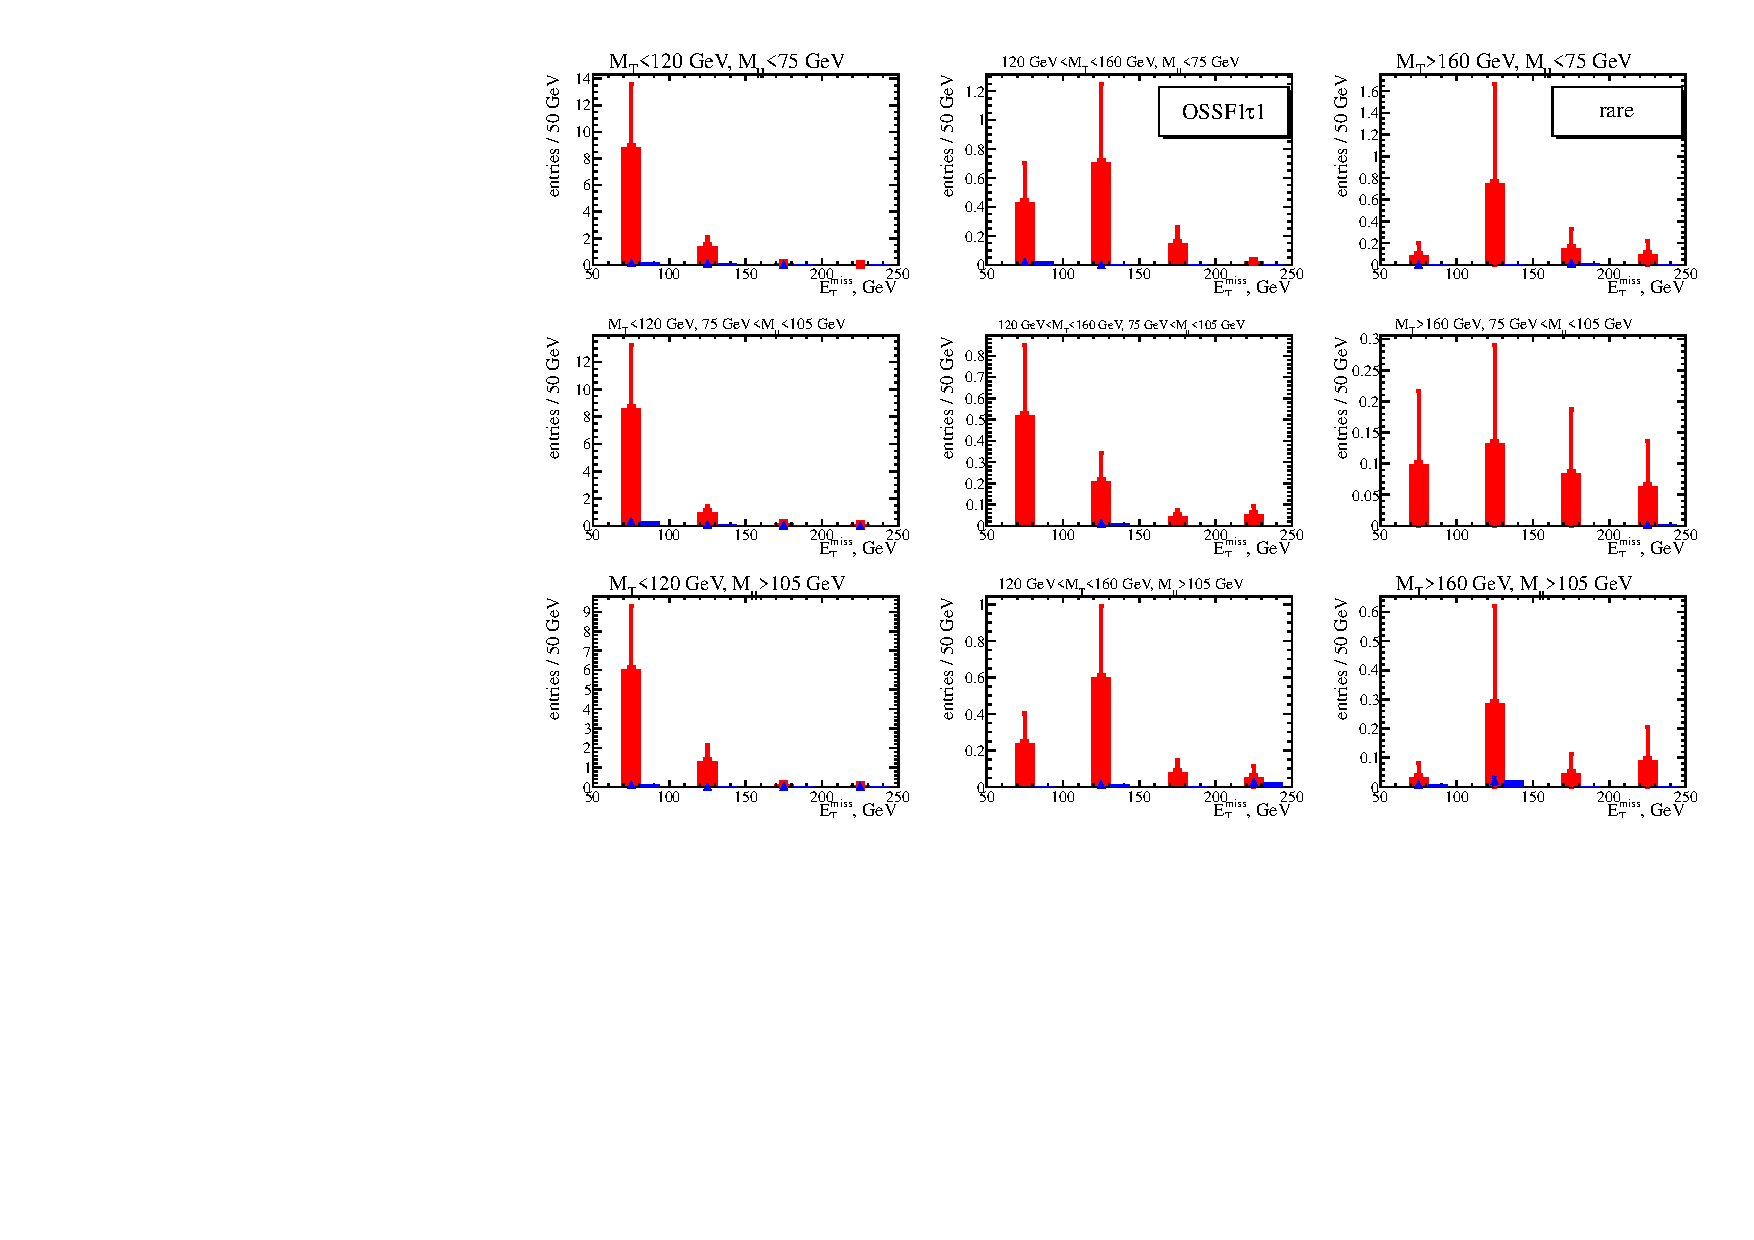
\includegraphics[width=1.0\textwidth]{plots/3lbkg/rare_ossf1tau1A.pdf}}
\caption{Comparison of the Rare SM contribution. Blue histograms from Ref.~\cite{AN2012:256} do not fully take into account 
all the processes therefore their contribution is excluded from the final combination.}
\label{fig:rare2}
\end{center}
\end{figure}
%==========================================================================================
%==========================================================================================
%==========================================================================================
\begin{figure}[htp]
\begin{center}
\subfigure[]
{\label{fig:wz_3l}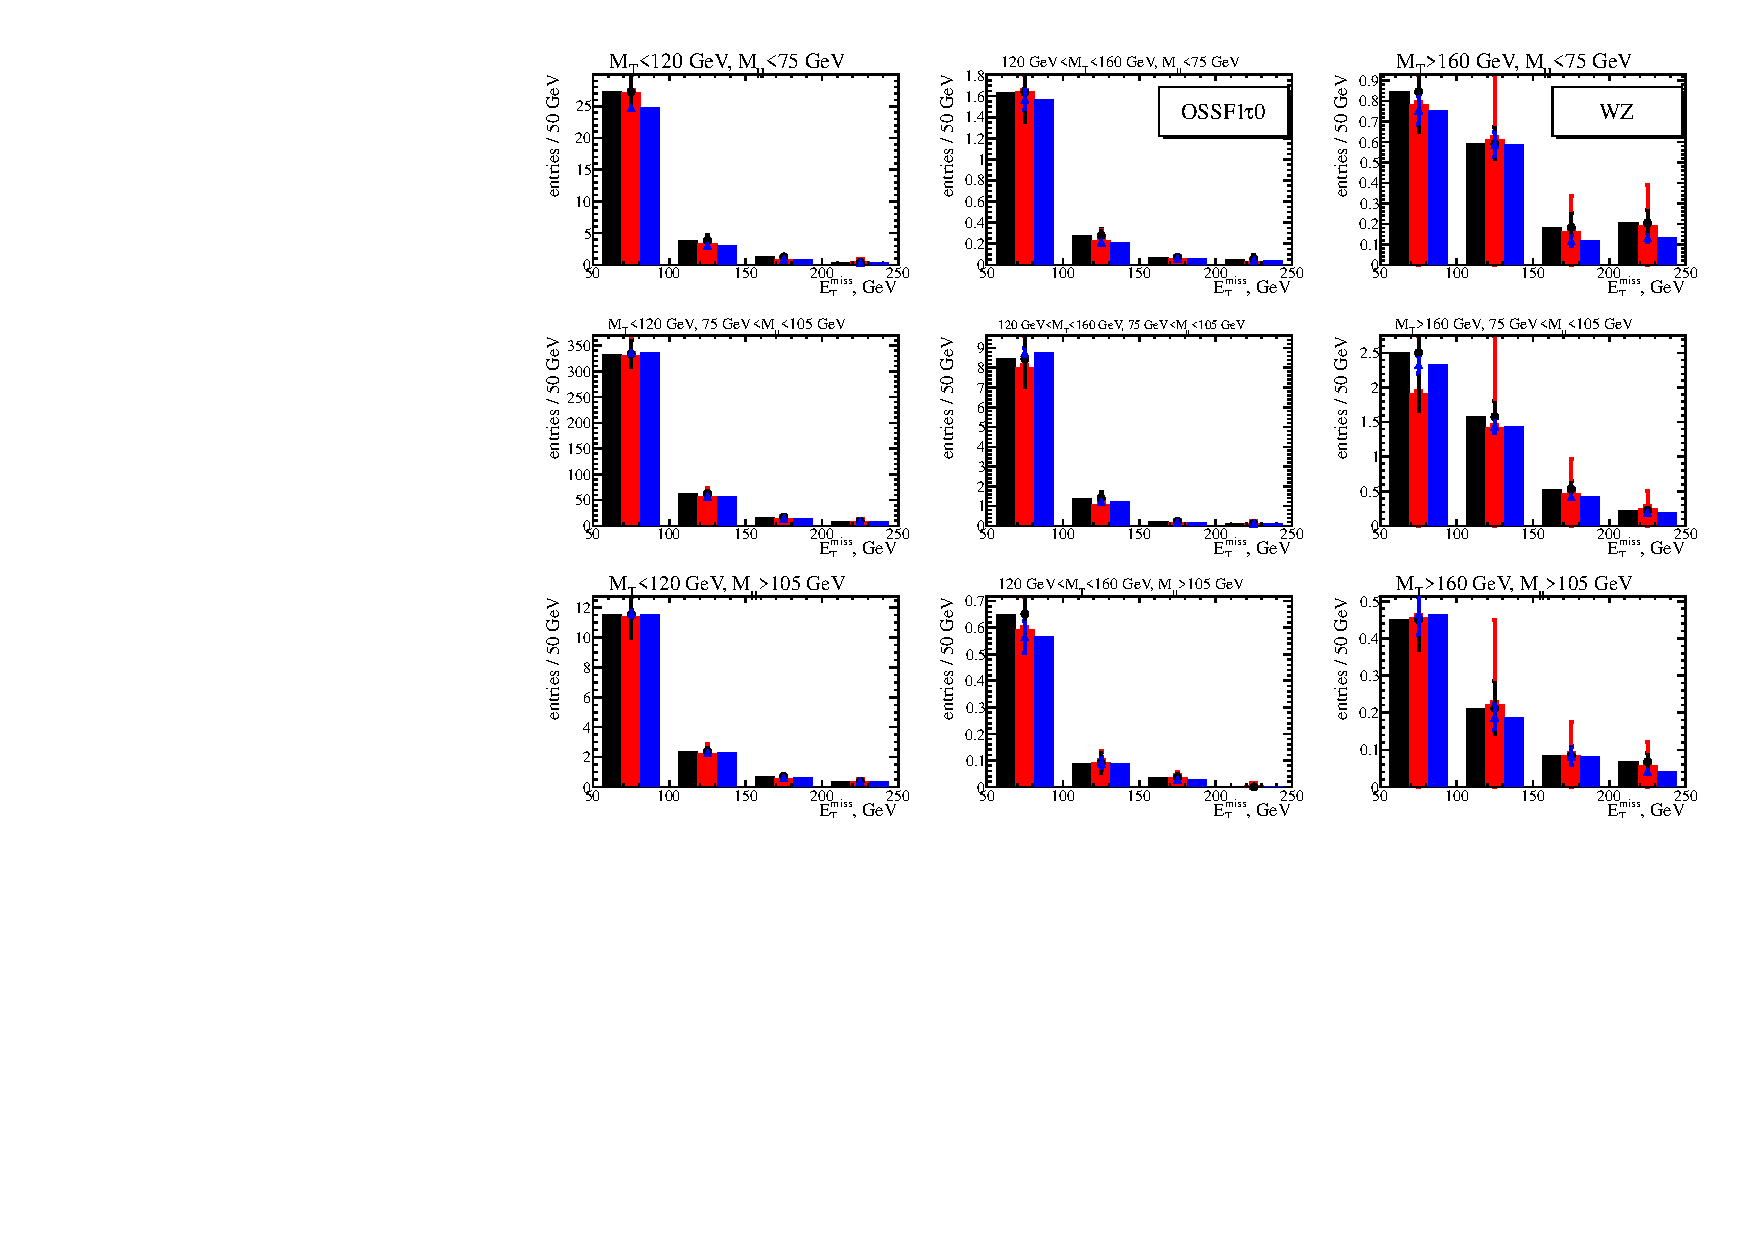
\includegraphics[width=1.0\textwidth]{plots/3lbkg/wz_ossf1tau0A.pdf}} \\
\subfigure[]
{\label{fig:wz_noOSSF}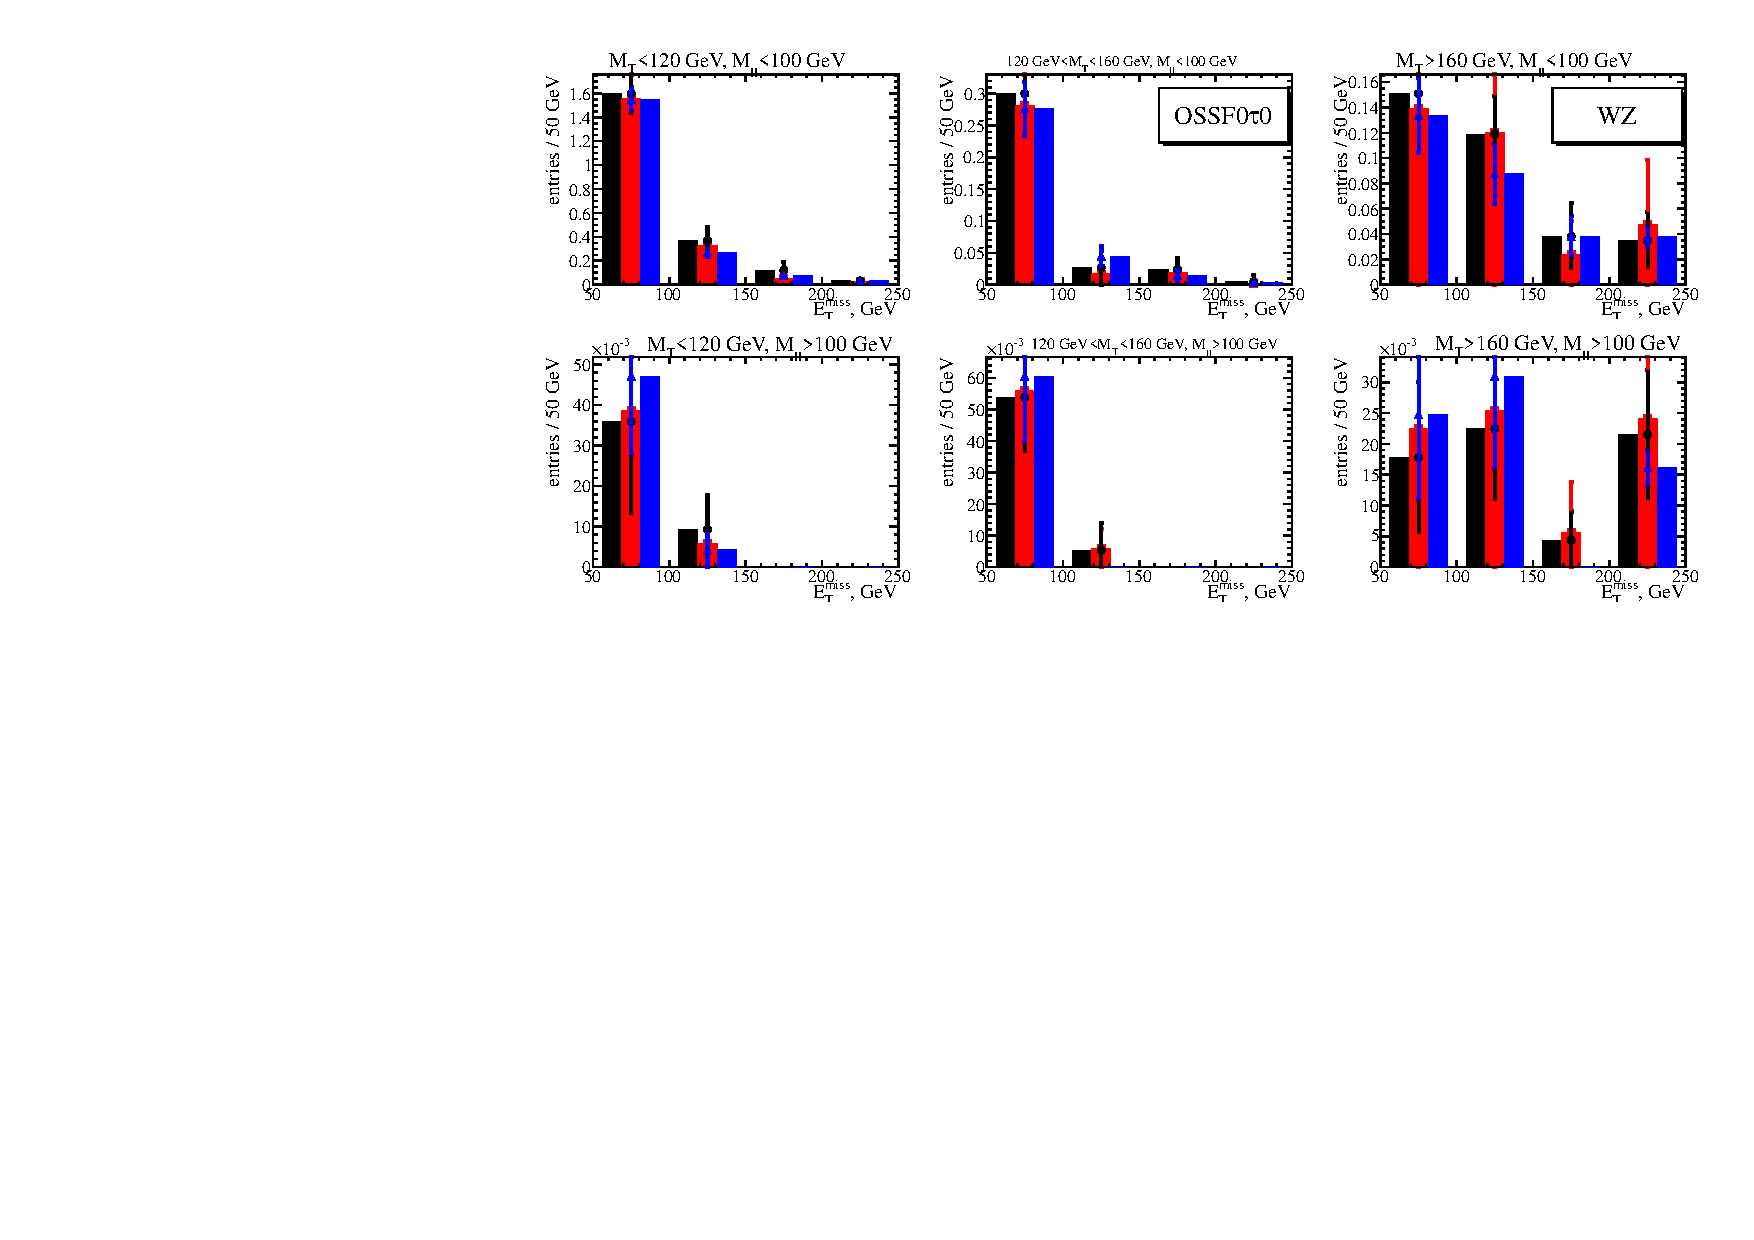
\includegraphics[width=1.0\textwidth]{plots/3lbkg/wz_ossf0tau0A.pdf}} \\
\caption{Comparison of the $WZ$ backgrounds.}
\label{fig:wz1}
\end{center}
\end{figure}
%==========================================================================================
%==========================================================================================
\begin{figure}[htp]
\begin{center}
\subfigure[]
{\label{fig:wz_SStau}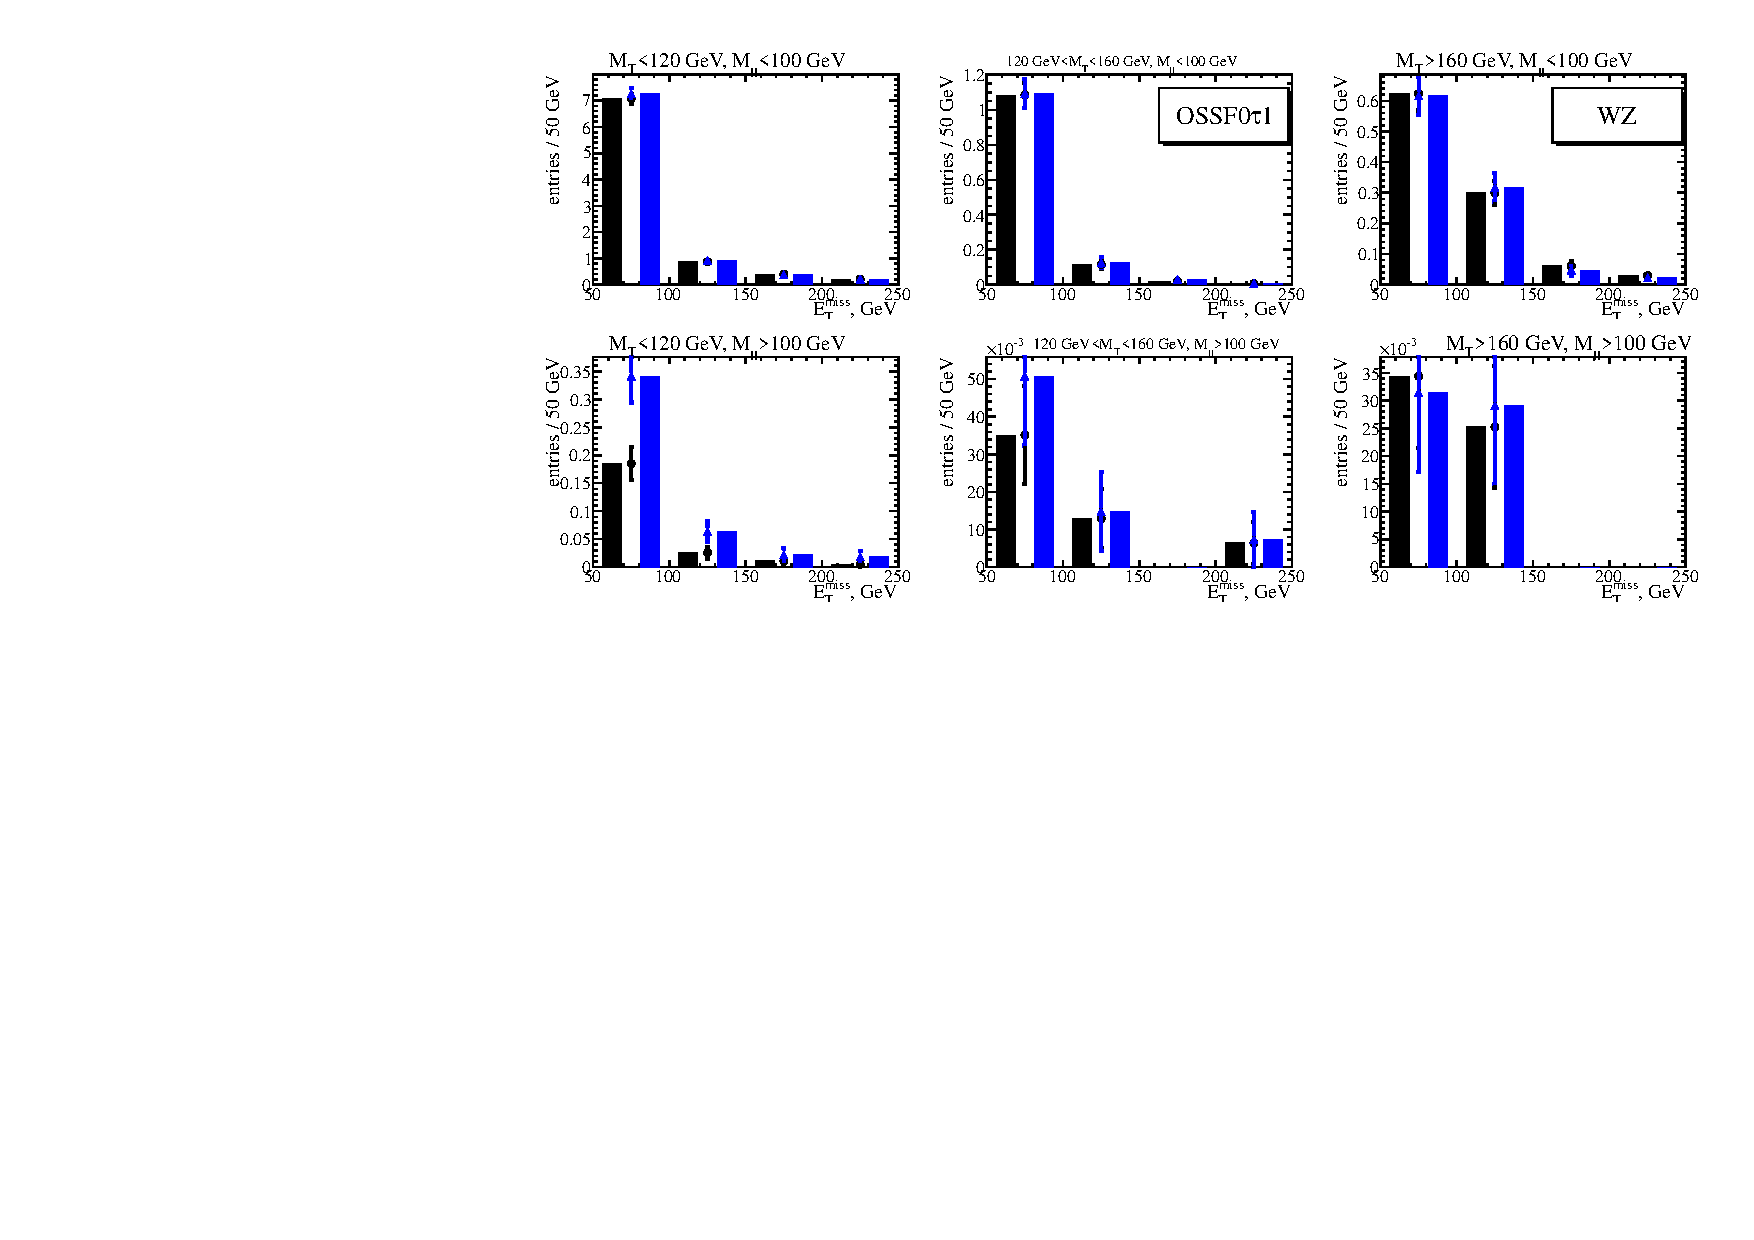
\includegraphics[width=1.0\textwidth]{plots/3lbkg/wz_ossf0tau1A.pdf}} \\
\subfigure[]
{\label{fig:wz_OStau}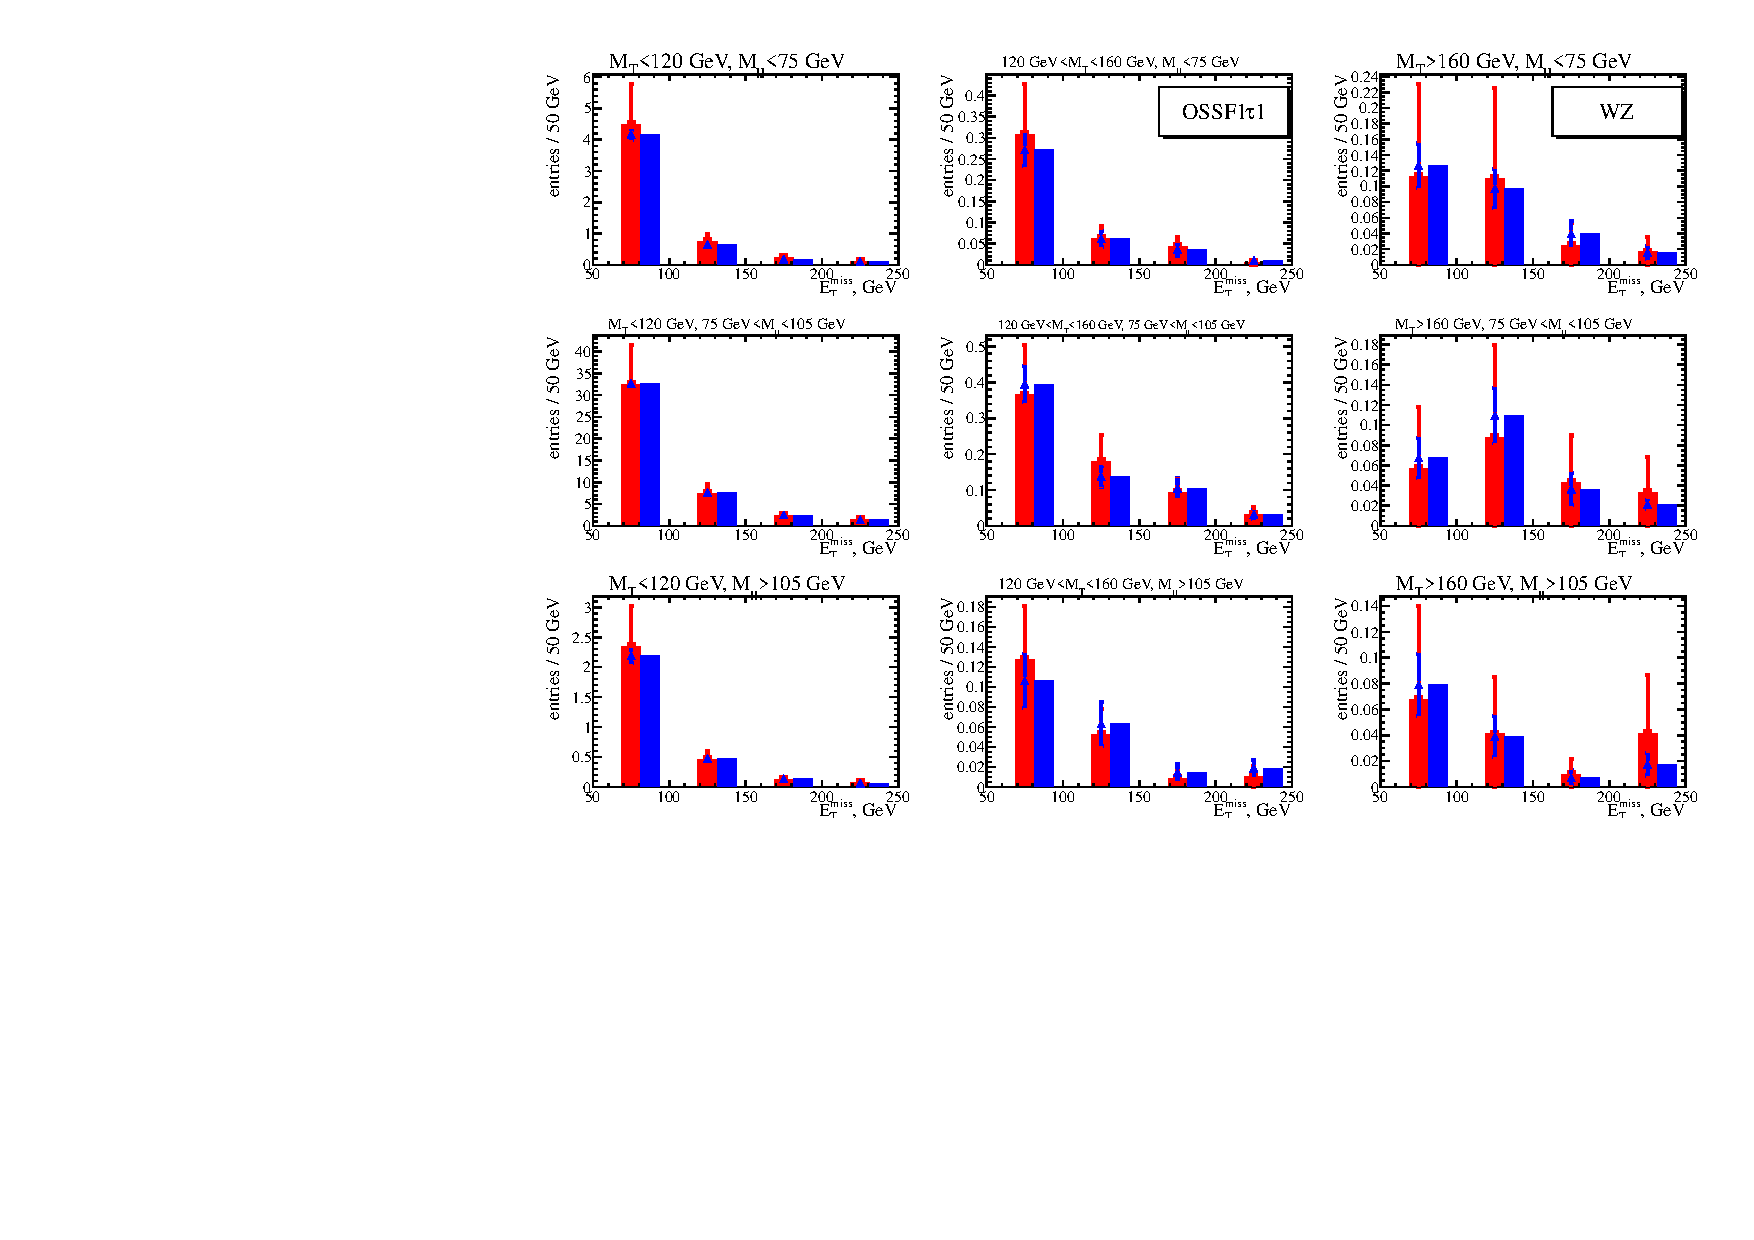
\includegraphics[width=1.0\textwidth]{plots/3lbkg/wz_ossf1tau1A.pdf}}
\caption{Comparison of the $WZ$ backgrounds.}
\label{fig:wz2}
\end{center}
\end{figure}
%==========================================================================================
%==========================================================================================
%==========================================================================================
\begin{figure}[htp]
\begin{center}
\subfigure[Non-prompt leptons legend.]
{\label{fig:tt_leg}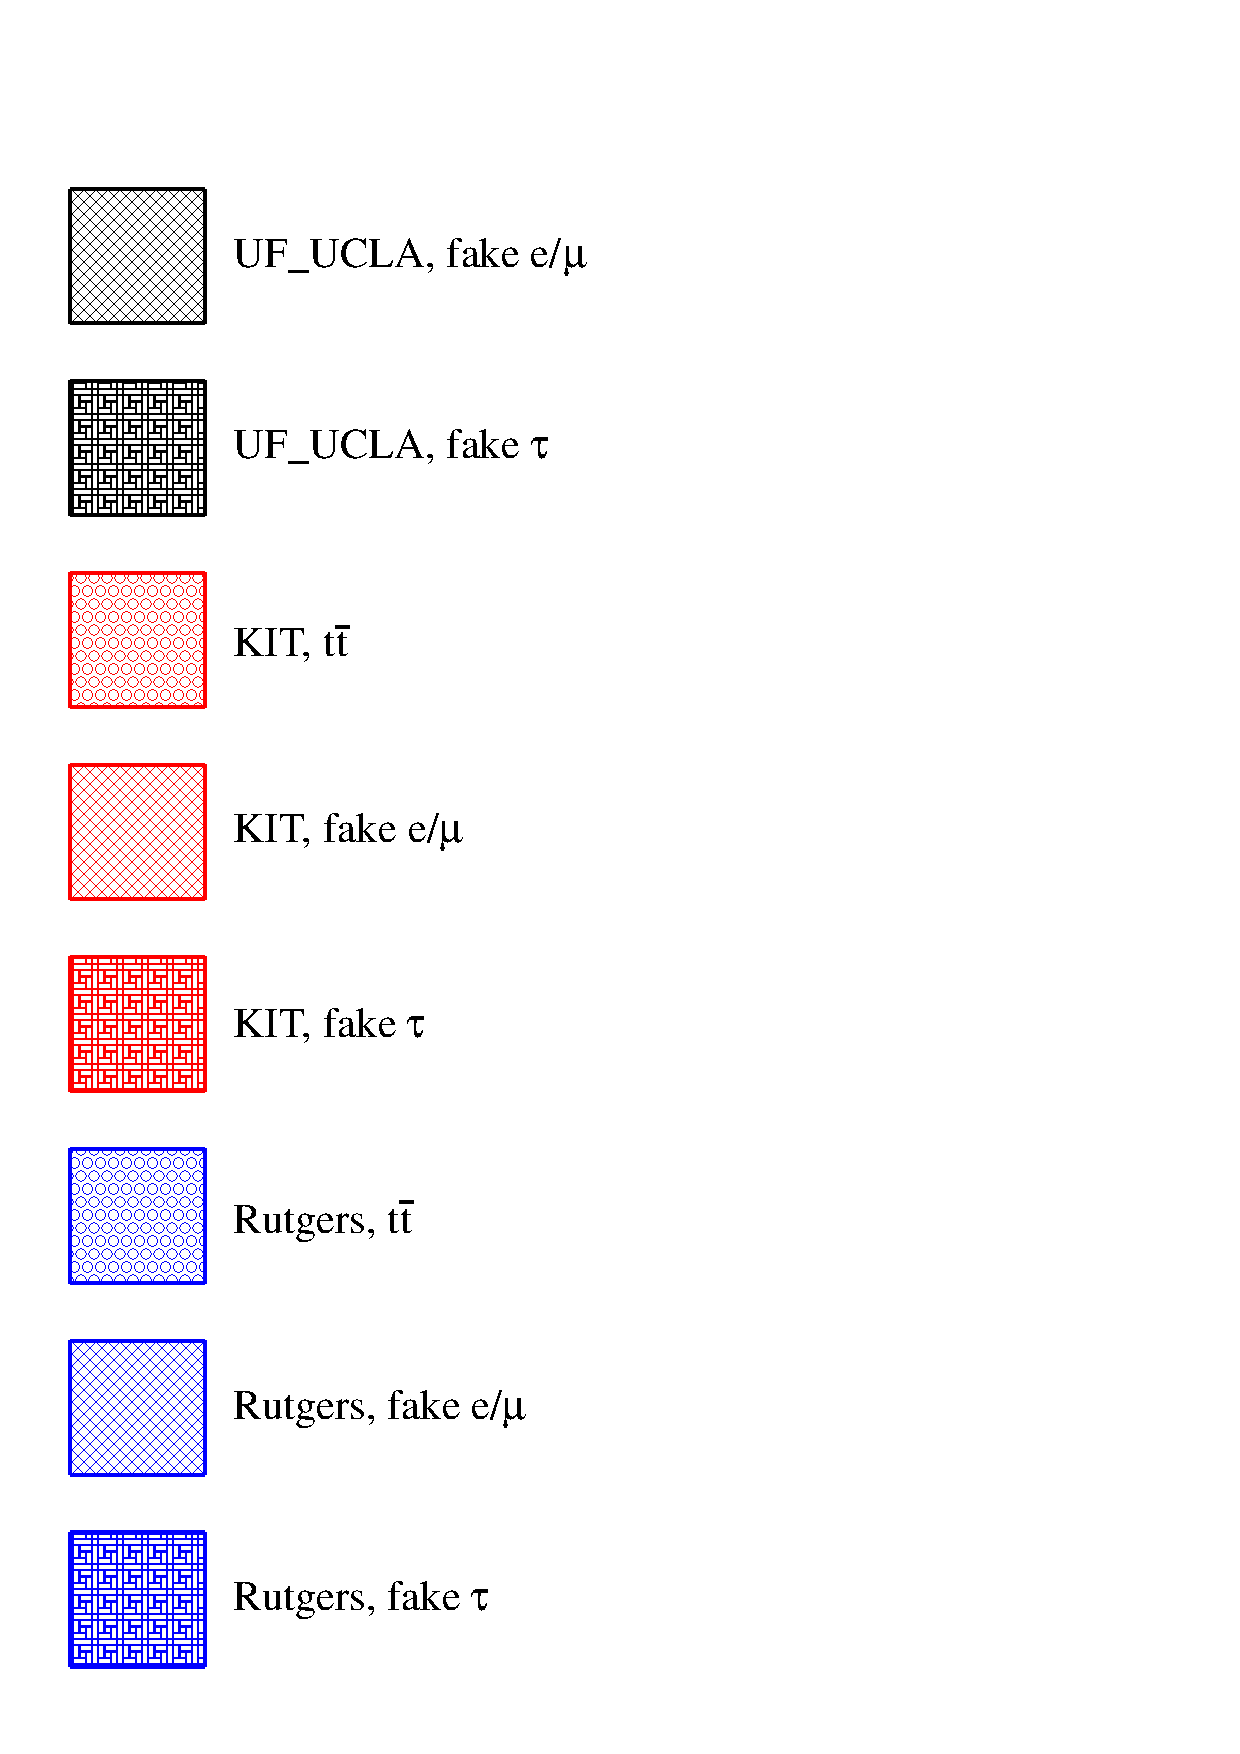
\includegraphics[width=0.5\textwidth]{plots/3lbkg/ttbar_legendA.pdf}} 
\subfigure[$ZZ$ and $Z\gamma^*$ legend.]
{\label{fig:zz_leg}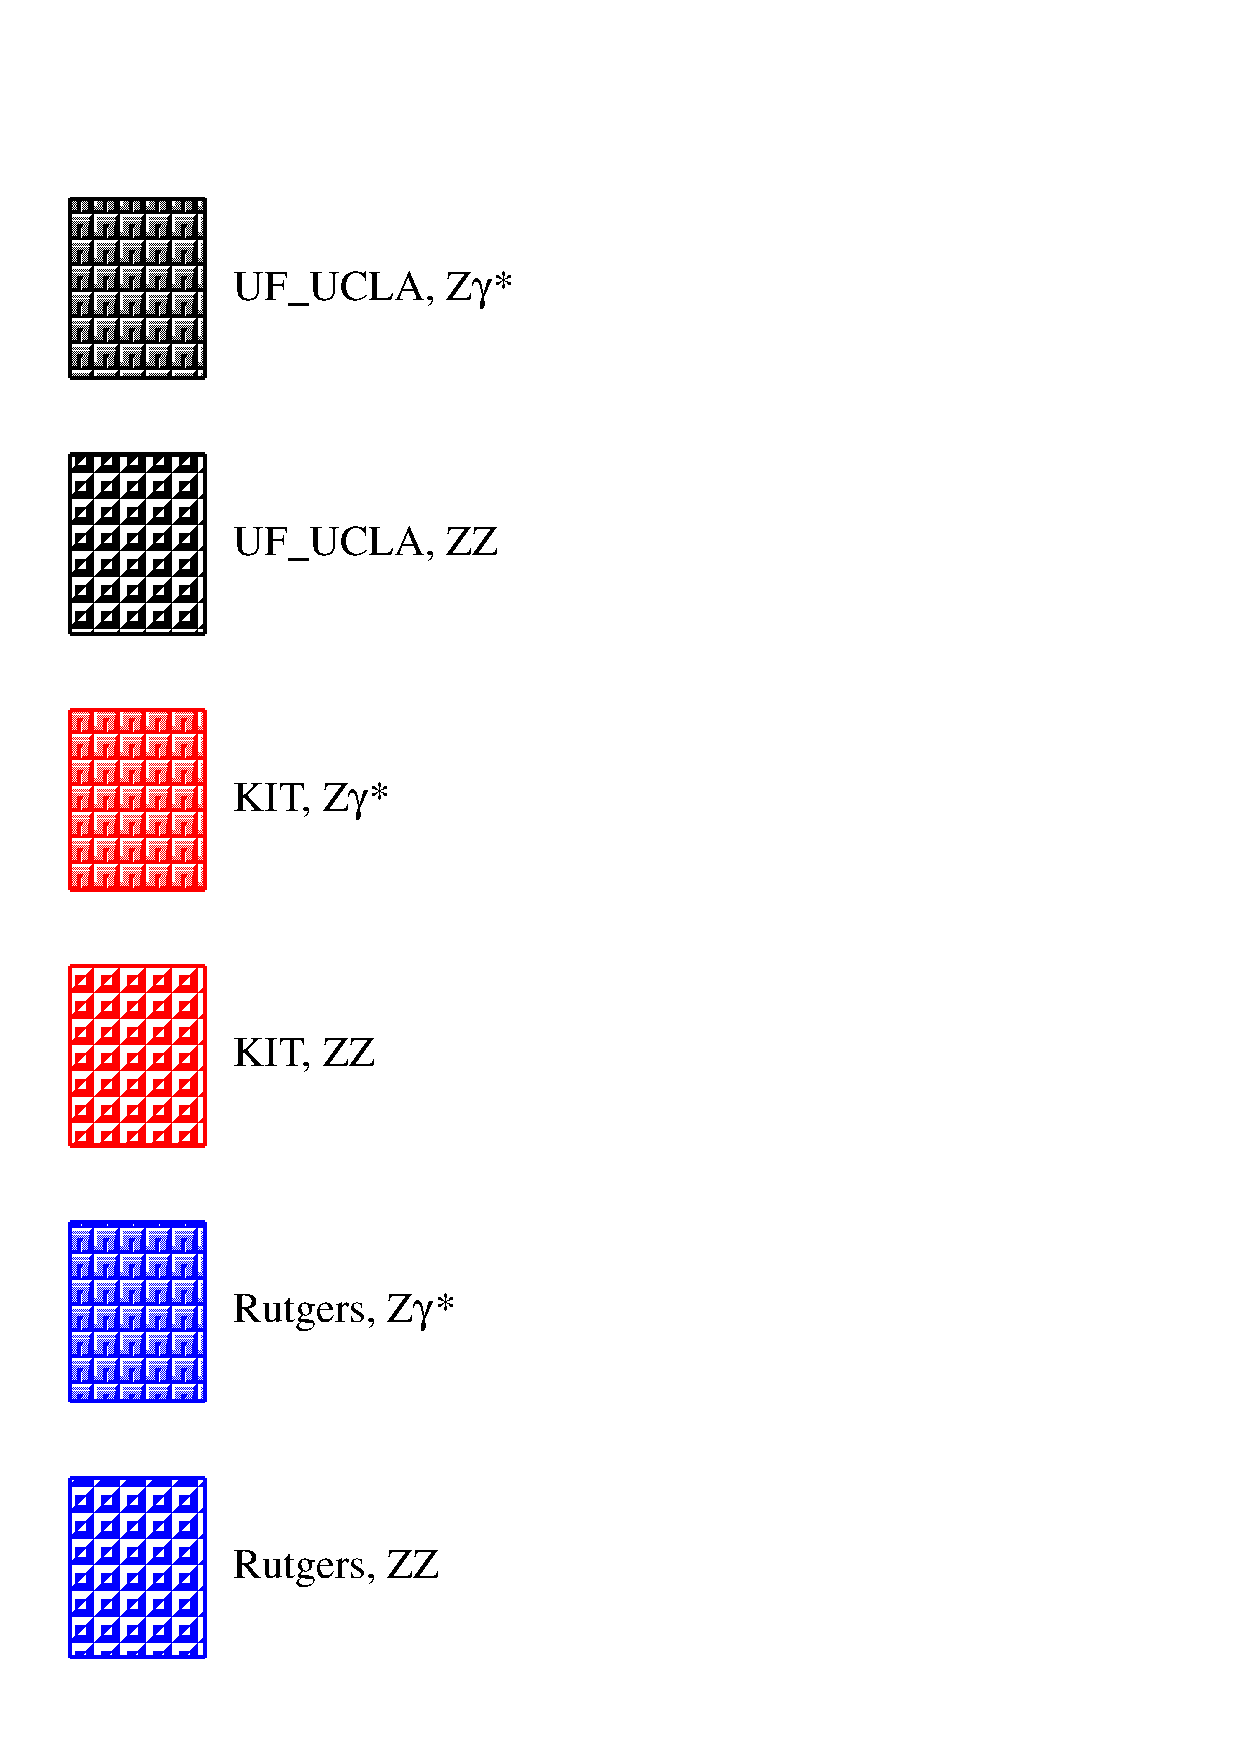
\includegraphics[width=0.5\textwidth]{plots/3lbkg/zz_legendA.pdf}} 
\caption{Legends for the following plots.}
\label{fig:legends}
\end{center}
\end{figure}
%==========================================================================================
%==========================================================================================
%==========================================================================================
\begin{figure}[htp]
\begin{center}
\subfigure[]
{\label{fig:zz_3l}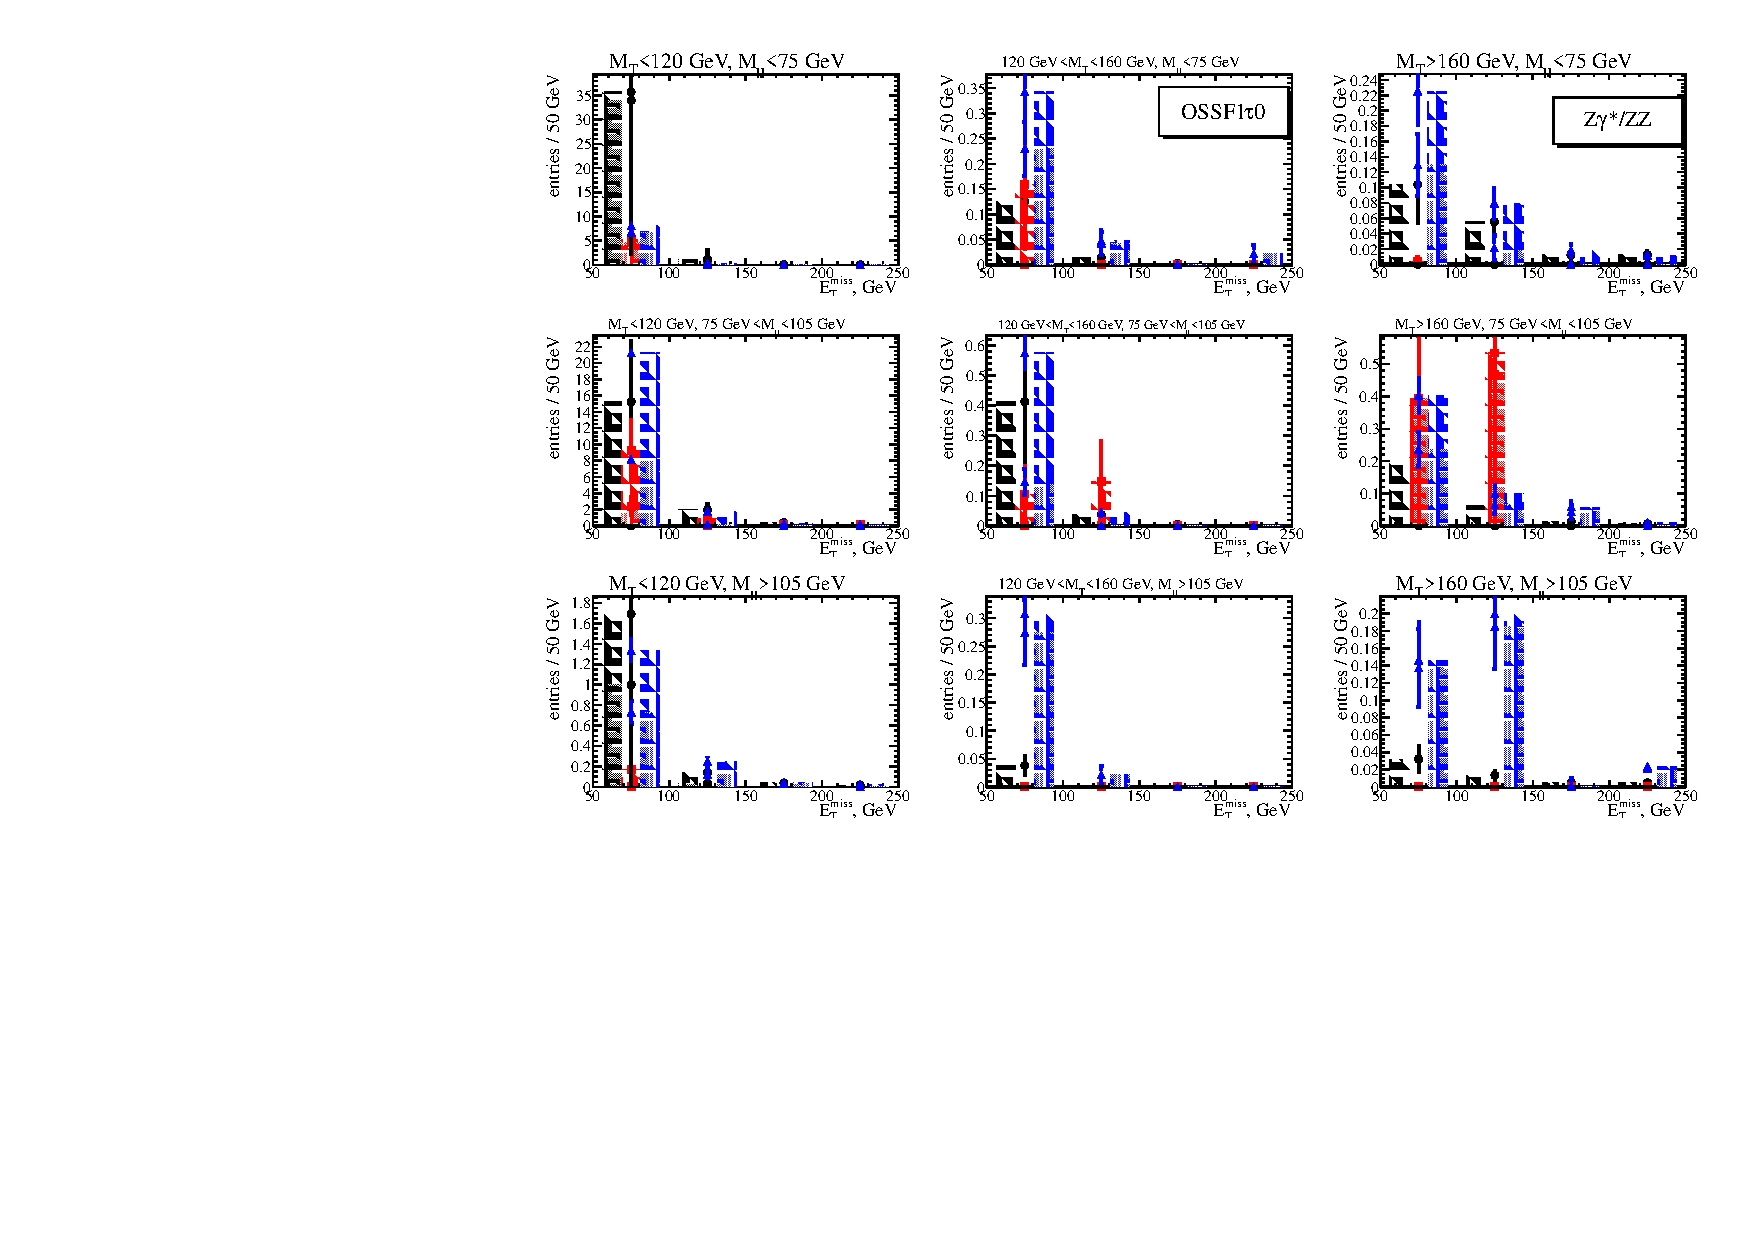
\includegraphics[width=1.0\textwidth]{plots/3lbkg/zz_ossf1tau0A.pdf}} \\
\subfigure[]
{\label{fig:zz_noOSSF}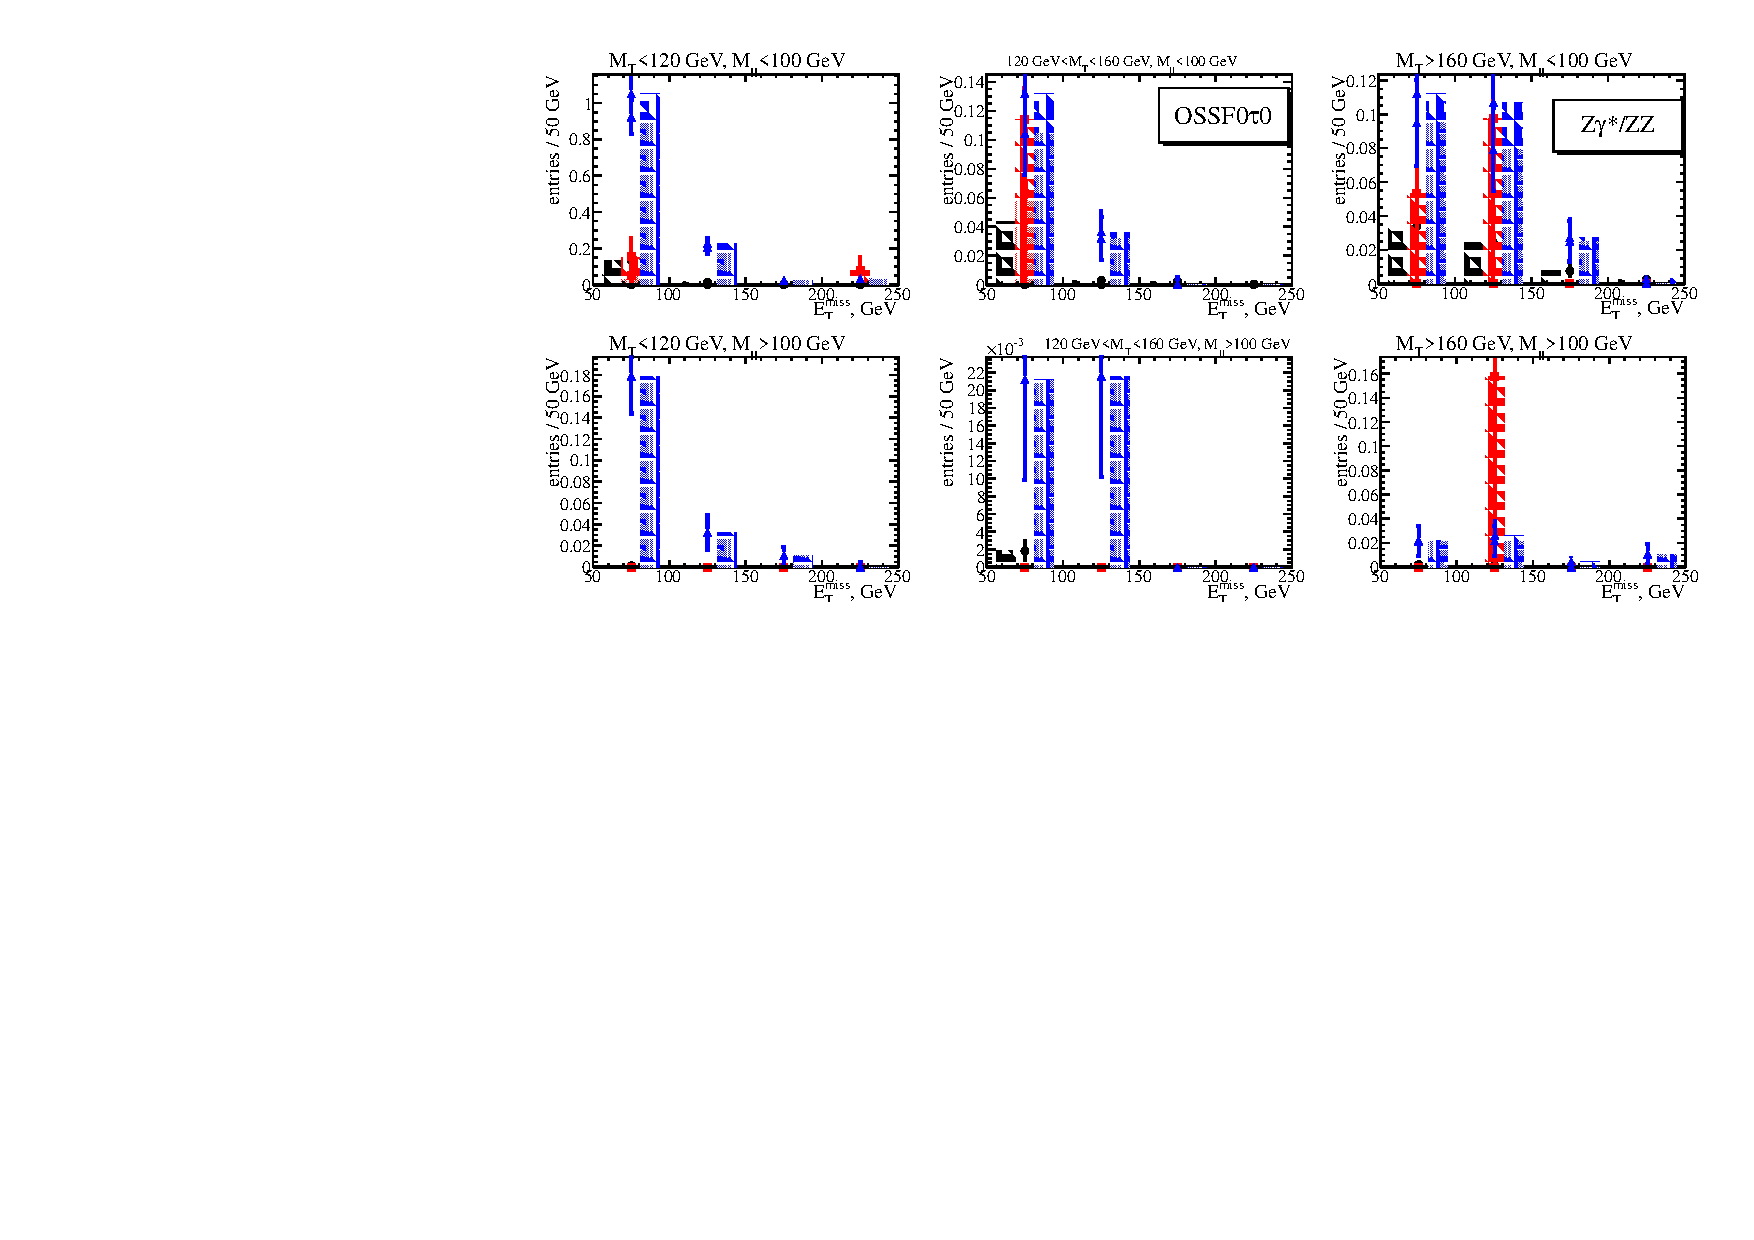
\includegraphics[width=1.0\textwidth]{plots/3lbkg/zz_ossf0tau0A.pdf}} \\
\caption{Comparison of the $ZZ$ and $Z\gamma^*$ contribution.}
\label{fig:zz1}
\end{center}
\end{figure}
%==========================================================================================
%==========================================================================================
\begin{figure}[htp]
\begin{center}
\subfigure[]
{\label{fig:zz_SStau}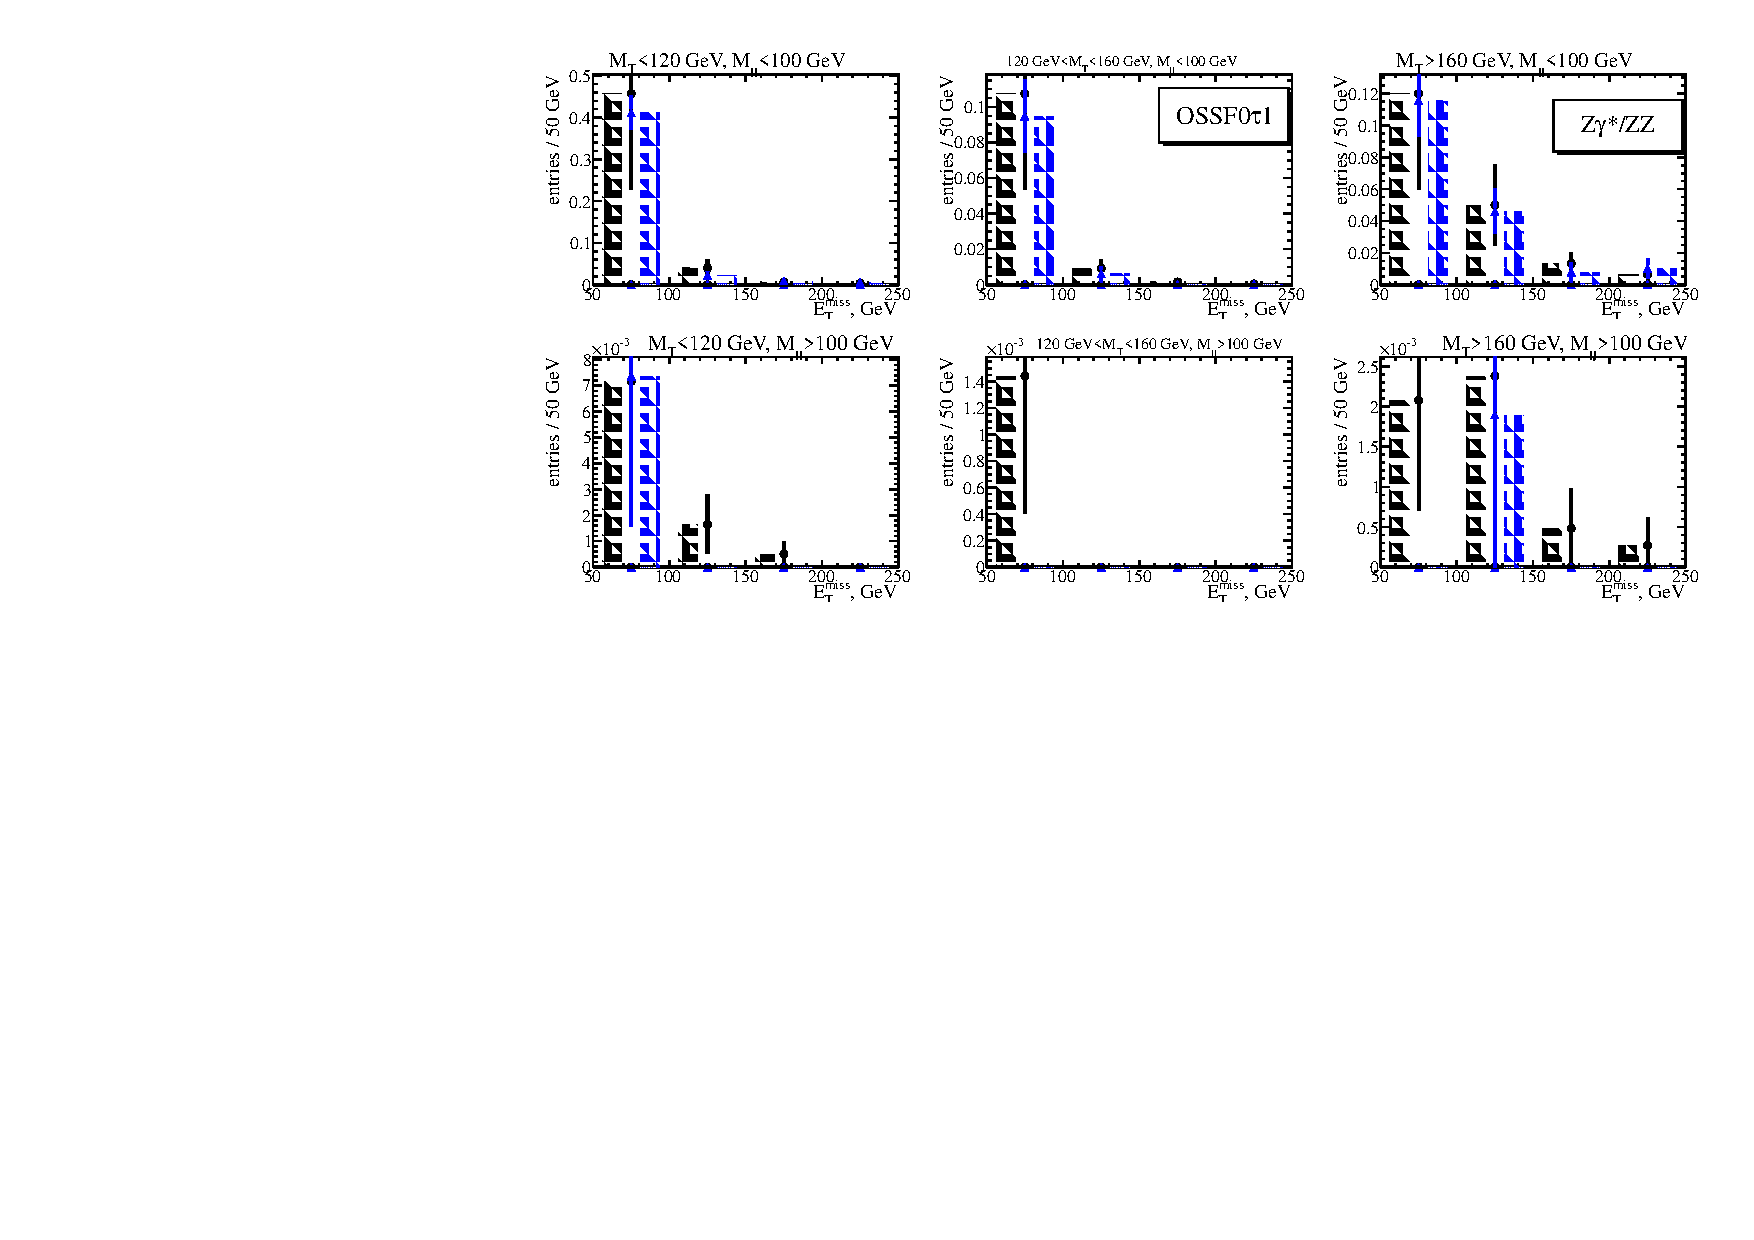
\includegraphics[width=1.0\textwidth]{plots/3lbkg/zz_ossf0tau1A.pdf}} \\
\subfigure[]
{\label{fig:zz_OStau}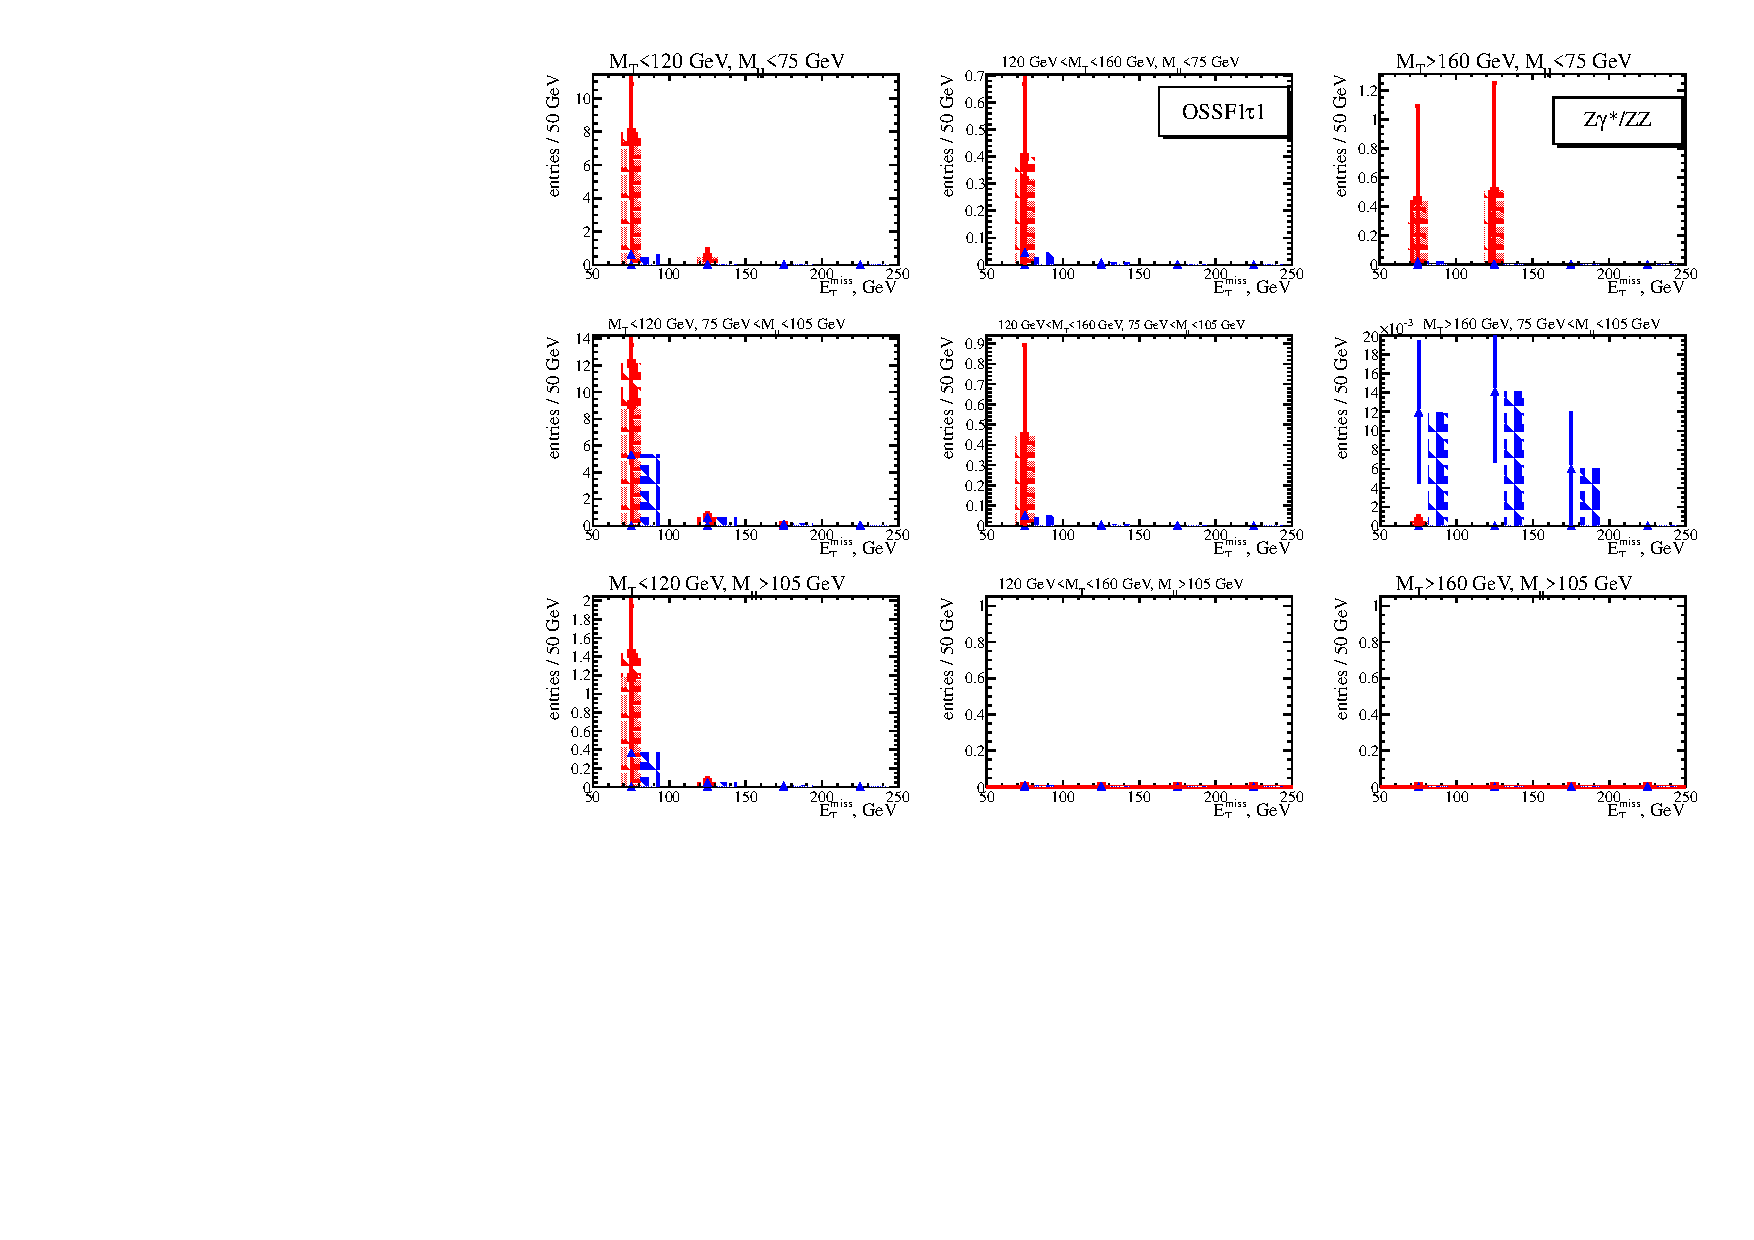
\includegraphics[width=1.0\textwidth]{plots/3lbkg/zz_ossf1tau1A.pdf}}
\caption{Comparison of the $ZZ$ and $Z\gamma^*$ contribution.}
\label{fig:zz2}
\end{center}
\end{figure}
%==========================================================================================
%==========================================================================================
\begin{figure}[htp]
\begin{center}
\subfigure[]
{\label{fig:fake_3l}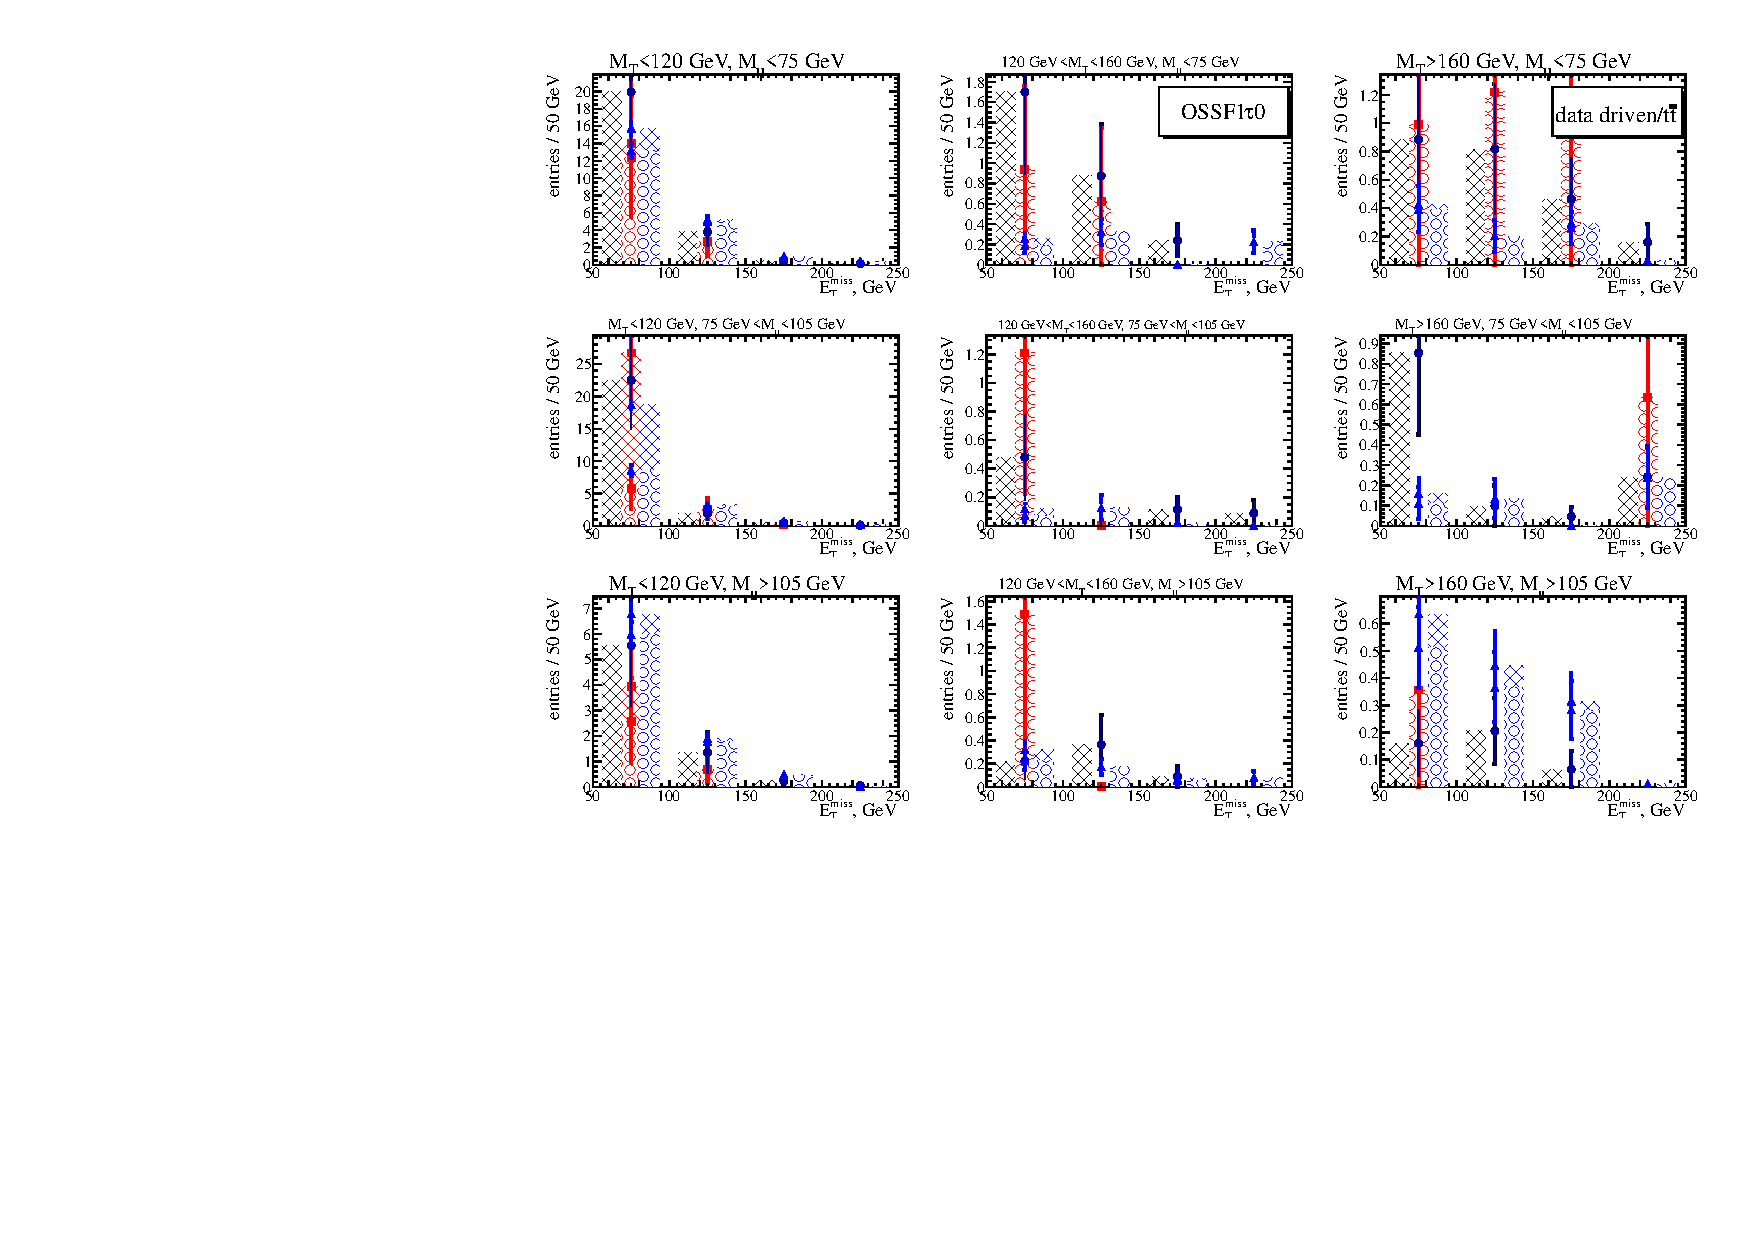
\includegraphics[width=1.0\textwidth]{plots/3lbkg/ttbar_ossf1tau0A.pdf}} \\
\subfigure[]
{\label{fig:fake_noOSSF}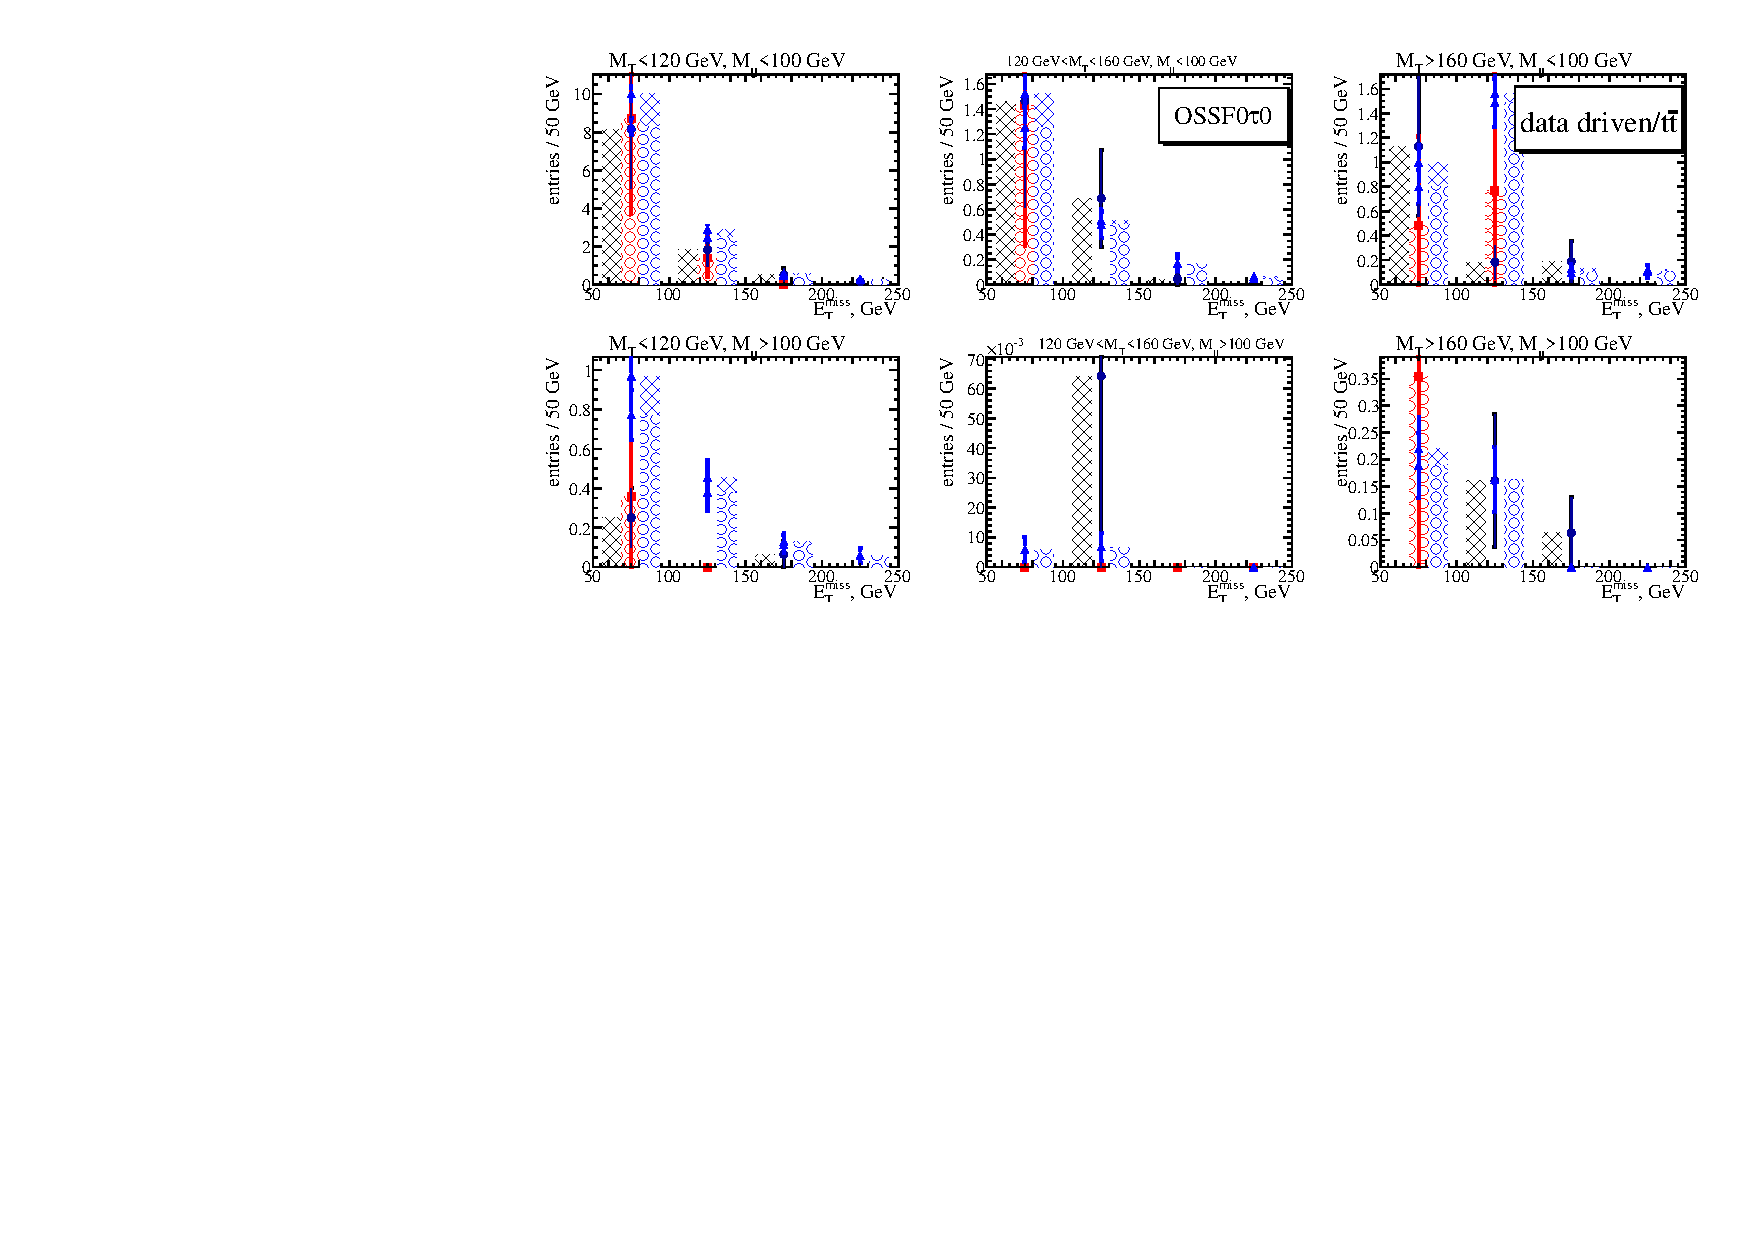
\includegraphics[width=1.0\textwidth]{plots/3lbkg/ttbar_ossf0tau0A.pdf}} \\
\caption{Comparison of the non-prompt leptons contribution.}
\label{fig:fake1}
\end{center}
\end{figure}
%==========================================================================================
%==========================================================================================
\begin{figure}[htp]
\begin{center}
\subfigure[]
{\label{fig:fake_SStau}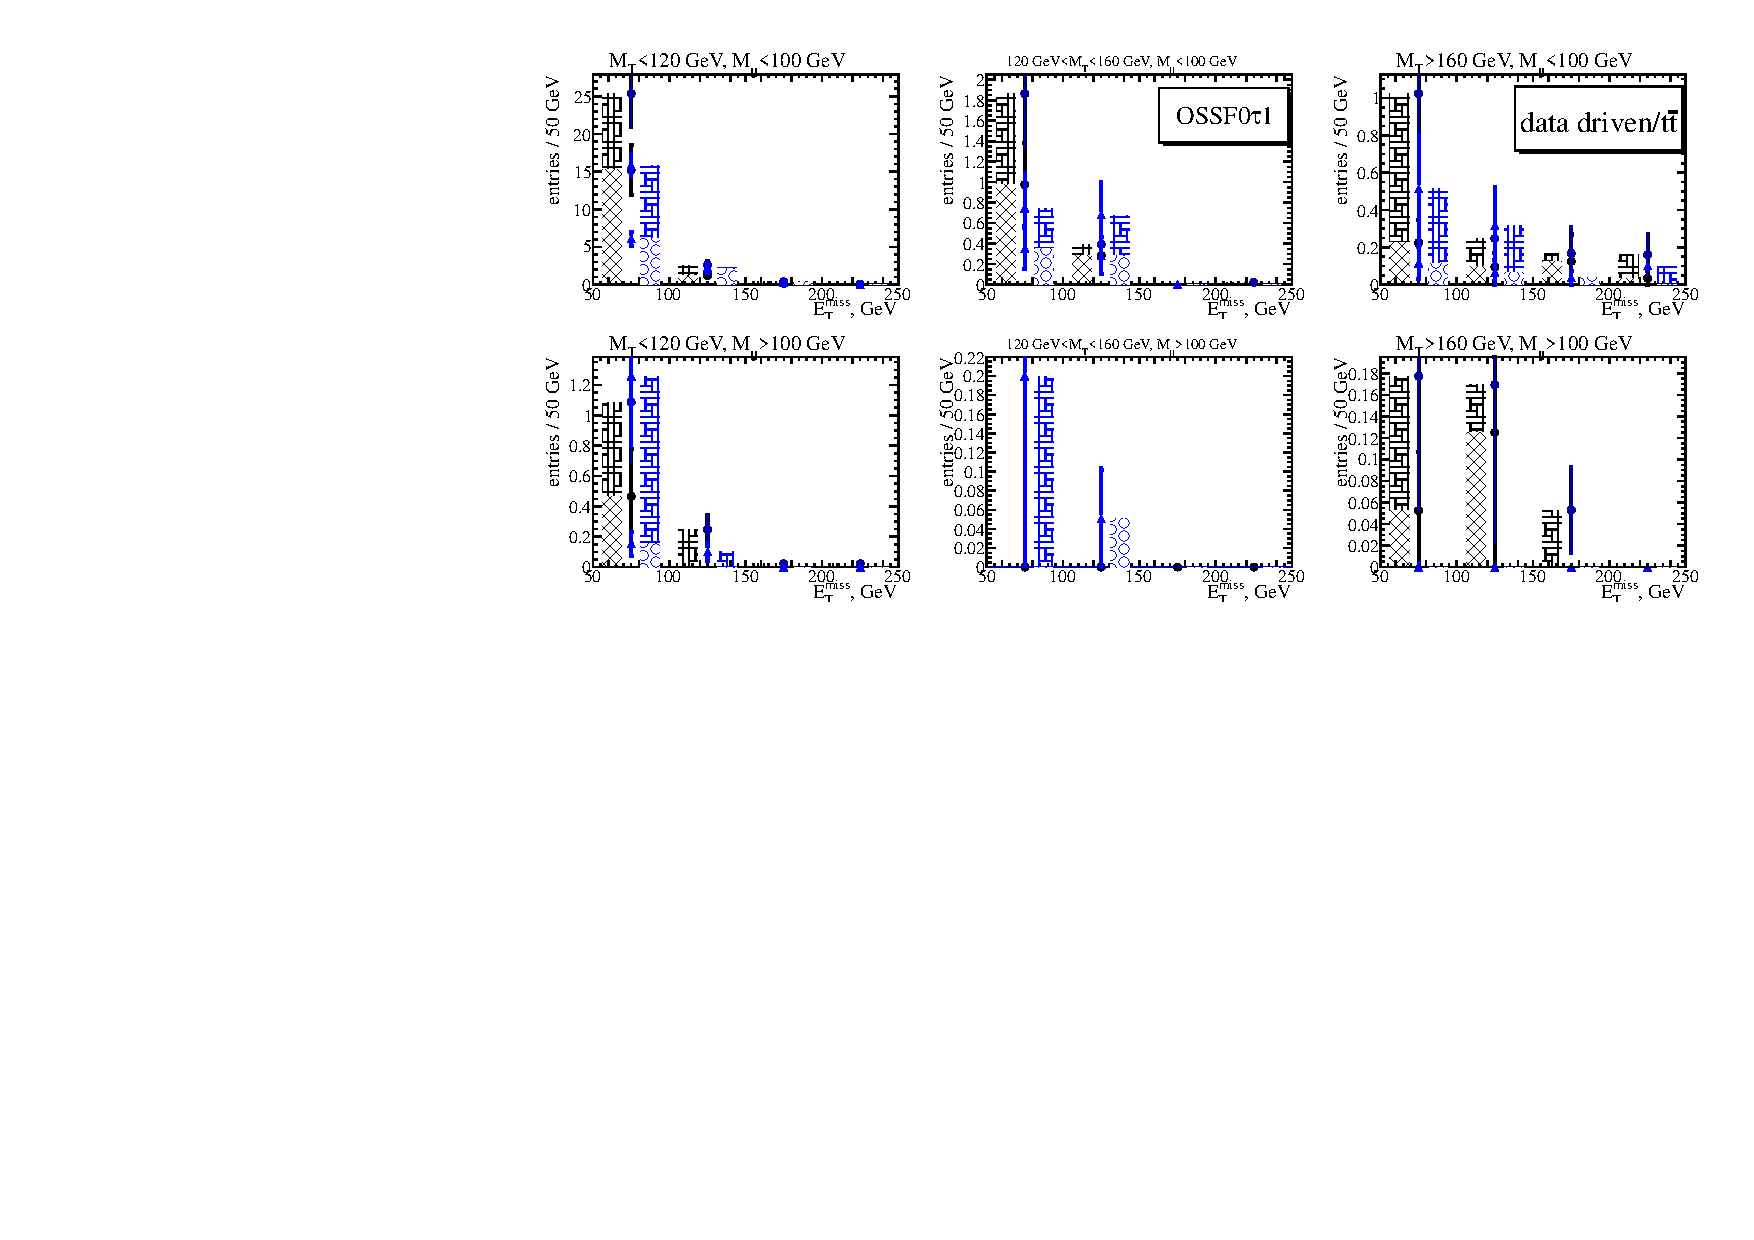
\includegraphics[width=1.0\textwidth]{plots/3lbkg/ttbar_ossf0tau1A.pdf}} \\
\subfigure[]
{\label{fig:fake_OStau}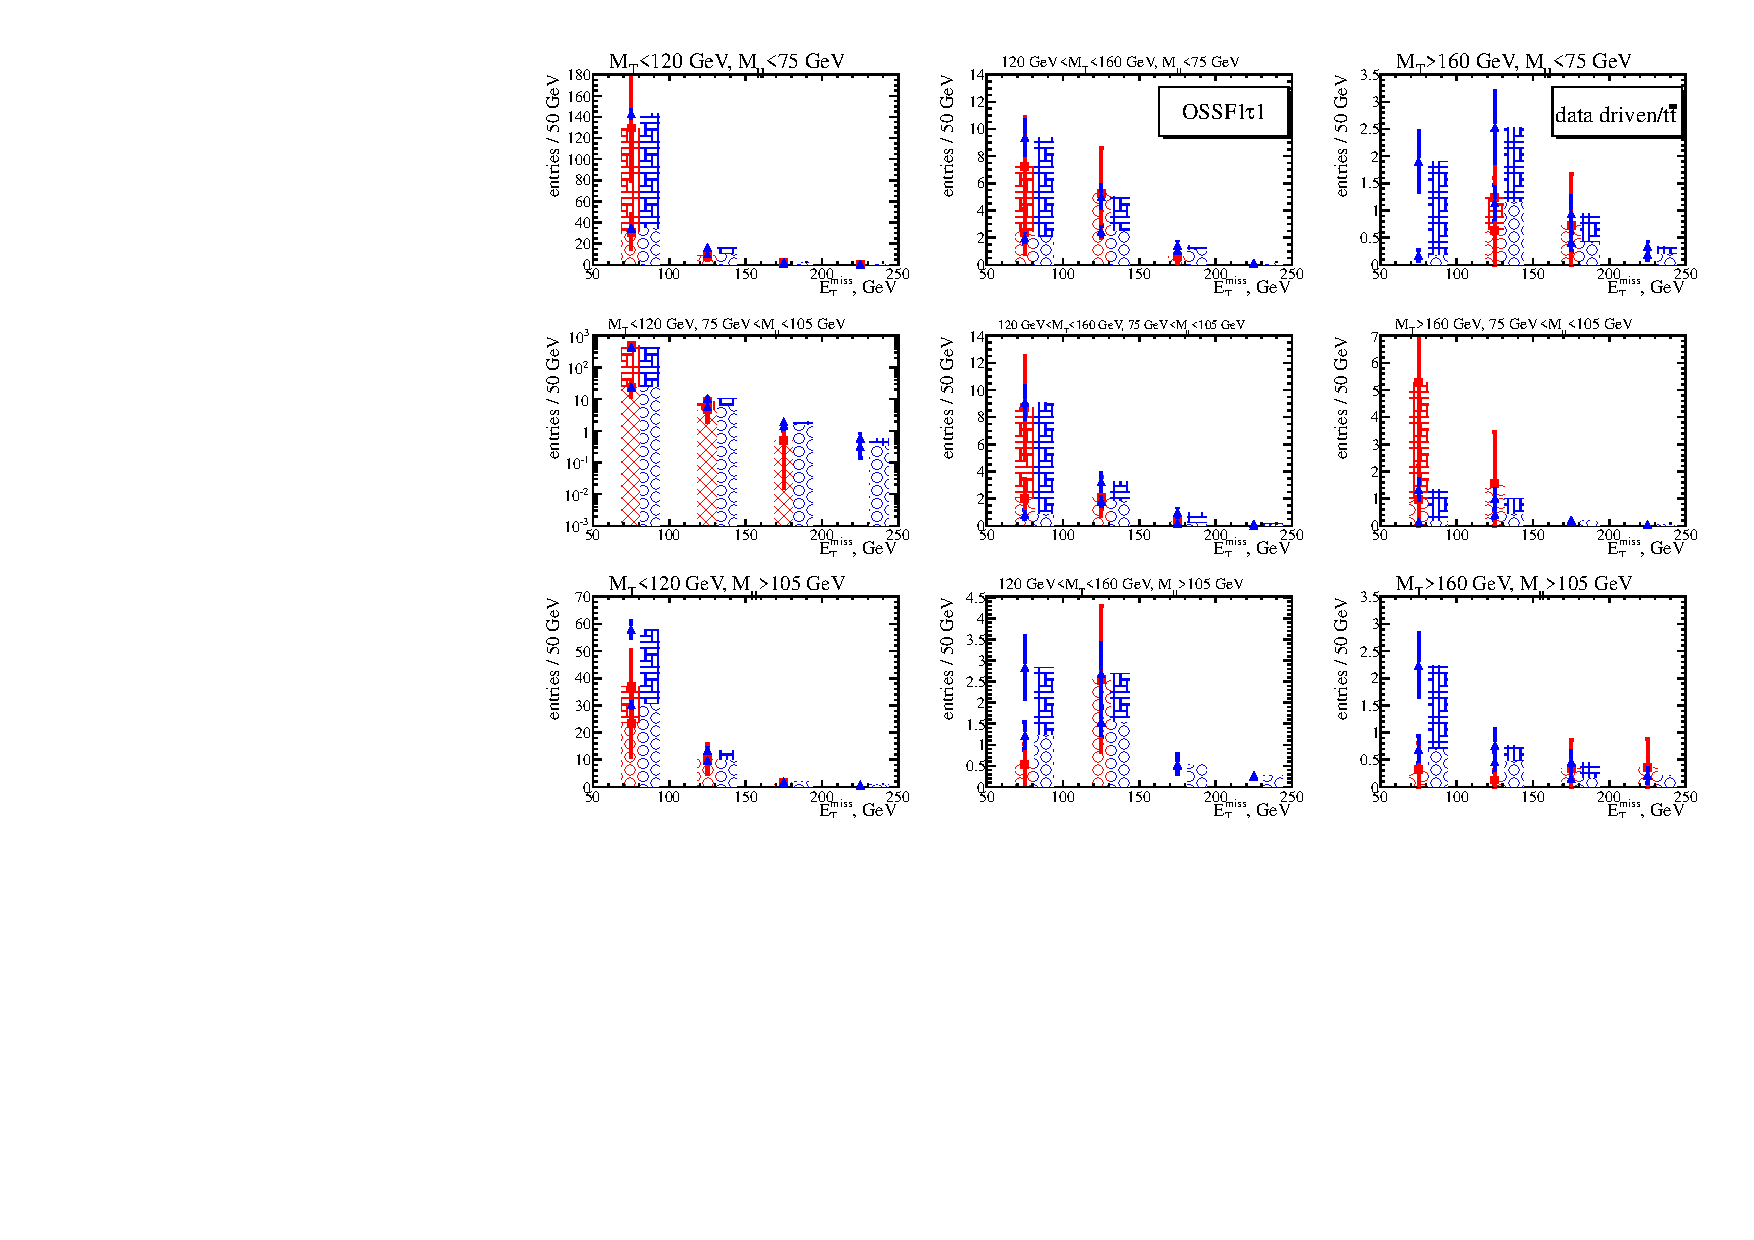
\includegraphics[width=1.0\textwidth]{plots/3lbkg/ttbar_ossf1tau1A.pdf}}
\caption{Comparison of the non-prompt leptons contribution.}
\label{fig:fake2}
\end{center}
\end{figure}
%==========================================================================================